% Note that if you want something in single space you can go back and
% forth between single space and normal space by the use of \ssp and
% \nsp.  If you want doublespacing you can use \dsp.  \nsp is normally
% 1.5 spacing unless you use the doublespace option (or savepaper
% option)
%
%(FORMAT) Usually you *don't* want to mess with the spacing for your
%(FORMAT) final version.  If you think/know that the thesis template
%(FORMAT) and/or thesis style file is incorrect/incomplete, PLEASE
%(FORMAT) contact the maintainer.  THANK YOU!!!

\chapter{INTRODUCTION}
\label{chap:intro}
A manned Mars mission places a heavy penalty on propellant inefficiency. This is because every kilogram of fuel required for landing must be delivered as payload through every phase of the mission until that point, and due to the exponential nature of Tsiolkovsky's rocket equation increasing landing payload mass is extremely expensive. The problem of powered descent guidance is then one of fuel optimality as well as safety, particularly in the case of a manned mission. 

% By labeling the chapter, I can refer to it later using the
% label.\:(\ref{chap:intro}, \pageref{chap:intro}) Latex will take care
% of the numbering.

\section{Guidance and Control in Aerospace} \label{sec:guidancevcontrol}
The powered descent guidance and soft landing problem under investigation is a problem requiring consideration of Guidance, Navigation, and Control principles and application. 

Guidance refers to trajectory planning of a vehicle to satisfy mission conditions and constraints. For the soft landing problem these conditions are the vehicle's initial state vector upon powered descent guidance initiation including its position and velocity, and the constraints are the desired final landing site, speed, and approach angle.

Navigation refers to the determination of the vehicle's state. For a manned Mars mission the navigation systems available may be restricted to an internal inertial navigation system (INS), which numerically propagates an estimate of the vehicle's state based on measured accelerations. The vehicle may also have various other sensors which provide updates to its INS state estimate to improve accuracy. These sensors include radar, barometers, and the like.

Control refers to the manipulation of forces to induce a desired trajectory, orientation, or change of state. For the soft landing problem these manipulations may be realized through aerodynamic surfaces, thrusters, rockets, or other systems which exert force on the vehicle.

This paper seeks to investigate the trajectory planning aspect of powered descent guidance for soft landing in the context of a manned Mars mission. It does not examine Control or Navigation strategies in detail, though it does illustrate their importance.

\section{Literature Review}
The problem of powered descent guidance has been studied extensively throughout the last century, particularly since The Space Race of the 1960s and the Apollo program which spawned E-Guidance, presented first in Cherry\:1964\:\cite{CHERRY}. These analyses have approached the problem in several different ways, but they generally share the requirement that the solution ensure soft landing in vacuum conditions. Most if not all of these analyses attempt to optimize fuel consumption due to the heavy penalty imposed on inefficient propellant use when landing on an extraterrestrial body. Almost all approaches also share the assumption of a fixed final time, computed or chosen in various ways. Few of them address the problem of powered descent initiation, or when to start powered descent guidance. None investigate powered descent initiation with E-Guidance in the context of a manned mission landing in atmosphere. Work has been done in mission phase planning but little optimization has been done for an  initial trajectory with free ignition time.

Cherry developed E-Guidance, of which Apollo Powered Descent Guidance (APDG) is a version. APDG solves the Equations of Motion\:(\ref{eqn:EoM1}) and\:(\ref{eqn:EoM2}) by defining a linear or quadratic thrust acceleration profile which ensures satisfaction of the terminal constraints\:(\ref{eqn:constraint_r}),\:(\ref{eqn:constraint_V}), and (for constrained final attitude)\:(\ref{eqn:constraint_a}). These two methods require choosing a fixed final time $t_f$, and Cherry proposes an algorithm similar to Algorithm\:(\ref{eqn:FPI}). The final time $t_f$ is dependent upon the initial conditions and assumes powered descent guidance is active.

D'Souza 1997\:\cite{DSOUZA} did consider an optimal time-to-go, the remaining flight time at any given moment of the powered descent trajectory. D'Souza's solution minimizes a weighted function of the time-to-go and the performance index given in Equation\:(\ref{eqn:performanceindex}. As discussed below, minimizing this performance index is not fuel optimal but by minimizing the time-to-go a better performance can be realized, as demonstrated in D'Souza's paper. However, this approach still only considers the problem after ignition, when the powered descent guidance phase has already begun.

Rea and Bishop 2010\:\cite{REA} examinded the fuel optimal powered descent guidance problem. They explored a time-to-go which optimizes their fuel optimal performance index, but it only considers the portion of flight after a deorbiting ``braking" maneuver which ends when the vehicle altitude reaches some pre-designated altitude. They also discuss the approaches previously explored and the limitations of these approaches. These approaches do not explore PDI optimization either.

Meditch 1964\:\cite{MEDITCH} showed that the fuel optimal thrust profile for a vertical landing given lower and upper thrust bounds is a ``bang-bang" style thrust, where the thrust switches between its upper and lower bounds with at most one switch between the bounds during descent. The paper examined the one-dimensional fuel-optimal powered descent in a uniform gravitational field. This strategy may be directly applicable for the final touchdown phase, during which the E-Guidance solution must be stopped when time-to-go gets small as discussed in Section\:\ref{sec:guidancecomp}.

Leitmann 1959\:\cite{LEITMANN} also examined a set of two-dimensional rocket flight problems including the two-dimensional powered descent and landing problem, similar to the problem under examination. Leitmann also showed that the fuel optimal thrust profile is ``bang-bang," with up to two switches.


\section{Contribution}
This paper seeks to improve upon APDG's fuel performance in the context of a manned Mars mission. The unique requirements of this mission include high payload mass, aerodynamics of the landing vehicle, critical safety requirements, and the very high penalty for propellant inefficiency. The method by which APDG is improved is through adaptive powered descent initiation (PDI) which enhances fuel efficiency by making use of a longer glide slope during which energy is shed through lift and drag effects without thrust while delaying ignition to reduce burn time and more closely approximate the optimal thrust profile. The solution presented is equally as computationally expensive as traditional E-Guidance and does not rely on high rate thrust magnitude switching. The guidance law has been studied extensively and flown on real spacecraft.

The strategy of Adaptive PDI is applicable beyond the implementation of APDG. This strategy is valid for any multi-phase mission involving powered descent and could be employed in many other contexts. It has particular applicability for atmospheric landings due to the increased efficiency gained from aerodynamic effects, safely extending the glide and aerobraking phase.

\section{Organization}
This thesis consists of a Methodology chapter in which equations are derived defining APDG and the Adaptive PDI strategy, a simulation chapter which details the simulation architecture and numerical implementation schemes used to test APDG and Adaptive PDI, a Results chapter in which the results of simulation are presented, a Discussion chapter in which the results are examined and interpreted, and a Conclusions chapter in which conclusions are drawn from the results and future work is recommended on the topic of Adaptive PDI.

Chapter\:\ref{chap:intro} introduces the soft landing problem and the motivation for Adaptive PDI. It defines the mission framework in which PDI is studied, and defines the powered descent guidance problem for derivation of APDG. It presents the relevant literature and prior work done on the topic of powered descent guidance and the contribution this thesis makes to that literature.

Chapter\:\ref{chap:methodology} derives E-Guidance and APDG, then presents the Adaptive PDI strategy and the relevant equations. It begins by defining the required notation and the coordinate frame used for the problem formulation.

Chapter\:\ref{chap:simulation} details the simulation architecture and numerical schemes used to implement Adaptive PDI with APDG and test its performance and robustness. The aerodynamic model is defined as well as the dispersion model for Monte Carlo testing. The initial conditions representing pre-determined Mars mission profile are given in Section\:\ref{sec:IC}.

Chapter\:\ref{chap:results} presents the results of simulation of the mission and makes several comparisons between various configurations. Section\:\ref{sec:PDIres} investigates the reliability of the Adaptive PDI strategy and its applicability for a practical mission. Section\:\ref{sec:lawcomp} compares the performance of APDG with E-Guidance, since APDG is less well tested and no claims are made about its optimality. Section\:\ref{sec:naverror} investigates the effects of navigation error. Sections\:\ref{sec:atmovsvac} through\:\ref{sec:atmoperf} presents results of simulation of a Mars mission and a similar mission in vacuum, comparing Adaptive PDI's performance to a traditional pre-determined ignition strategy. 

Chapter\:\ref{chap:discussion} discusses the results of Chapter\:\ref{chap:results} and verifies the simulation output through error analysis.

Chapter\:\ref{chap:conclusions} states the conclusions of the study and makes recommendations for future study of the Adaptive PDI strategy.

%You can save yourself 12 minutes now by not reading this document;
%later on the average payback is 105-fold when you run into problems.

%\section{History}
%
%In the early 1990s Richard Frost put together a \LaTeX style file for
%SDSU theses based on \LaTeX~2.09.  Joe Mahaffy wrote an example thesis
%to guide students in the use of \LaTeX\ code.  Since that time \LaTeX
%has been upgraded to \LaTeX2$\epsilon$ and the formatting requirements
%for SDSU have also changed.  In 2004, Jiri Lebl and Mike O'Sullivan
%worked on a revision, upgrading to \LaTeX2$\epsilon$.  This
%\LaTeX2$\epsilon$ class file basically has almost nothing in common
%with the old \LaTeX\ style; it is a modification of the standard
%report class.
%
%The class file \verb+sdsu-thesis.cls+ and this example are/have been
%maintained by
%\begin{itemize}
%\item Aug 2010 --- \emph{current}: Peter Blomgren,
%  \verb+<blomgren.peter@gmail.com>+.
%\end{itemize}
%
%In September 2010, the ``short'' example was merged into the ``long''
%example to form this document; this seemed like a reasonable thing to
%do.
%
%While every effort is/has been made to make sure that the template and
%thesis style conforms to the \emph{SDSU Thesis Manual}, \textbf{no
%guarantees can be made.}  Depending on the thesis reviewer and his/her
%interpreation of what is Really Important$^{\hbox{\scriptsize TM}}$ in
%the thesis manual, and his/her level of caffeination some theses fly
%through, and some get stuck even though they use the same template and
%style file.
%
%PLEASE let the maintainer know of any and all feedback you get from
%the thesis reviewer so that the template and/or style file can be
%updated as necessary.  THANK YOU!!!
%
%
%\section{Purpose}
%
%This document illustrates some of the typesetting tasks that are
%commonly encountered in a thesis containing
%mathematics\footnote{\texttt{http://en.wikibooks.org/wiki/LaTeX}\quad
%  provides a wealth of information regarding \LaTeX, check it out.}.
%All theses must follow the guidelines of the SDSU Thesis Manual for
%formating.  Most formating issues will be automatically handled by the
%\LaTeX\ class file included with the source file for this document,
%but there may be some special circumstances that will require some
%tinkering with spacing, pagebreaks, etc.
%
%\LaTeX\ is a remarkably powerful package, but it does take some effort
%to learn.  The best plan is to start with something already written
%and learn from the example.  The current document was produced for
%this purpose.  This document illustrates how the student should format
%the chapters and sections of the thesis, prepare the bibliography, and
%include other appropriate items commonly found in a technical
%document.  The title page, signature page, acknowledgments page,
%abstract, and everything else are all formatted according to
%specifications of the SDSU Thesis Manual of 2004, once you enter the
%text to include.
%
%For a general reference it is recommended that the student obtain the
%user's guide and reference manual of Leslie Lamport\:\cite{LAM}. The
%student should obtain copies of the files used to generate this
%document, then examine the ASCII files used to generate the document
%and the \LaTeX\ output.  The files for this example thesis are the
%following.
%\begin{itemize}
%\item \verb+Makefile+: Contains ``recipes'' for building the thesis;
%  type typing \verb+make+, and \verb+make thesis.pdf+.
%\item \verb+abstract.tex+: Contains the abstract.
%\item \verb+append.tex+: Contains all the text for appendices.
%\item \verb+body.tex+: Contains all the text for chapters. 
%\item \verb+sdsu-thesis.cls+: Defines the layout and formatting.
%\item \verb+thbib.bib+:  Contains a bibliographical database.
%\item \verb+thesis.tex+: 
%  \begin{enumerate}
%  \item  Contains information for the title page, and other
%    front-matter.
%  \item Includes the files \verb+abstract.tex+,  \verb+body.tex+, and
%    \verb+append.tex+. 
%  \item Defines the bibliographical style (\verb+siam+ in this
%    example) and creates the bibliography using the file
%    \verb+thbib.tex+.
%  \end{enumerate}
%\item \verb+cos.eps+, \verb+mapping.eps+, \verb+plot2.eps+, and
%  \verb+somb.eps+: Encapsulated postscript files that are included by
%  \verb+body.tex+ (in the subdirectory \verb+Figures/+.)
%\end{itemize}
%
%Positioning and captioning of figures and tables should agree with the
%thesis manual.  Occasionally, \LaTeX\ does not break when you want it
%too, so you have to add a \verb+\newpage+ command to get
%the correct break, such as when a section header starts at the bottom
%of a page or when paragraphs have widows or orphans.
%
%
%\section{Format of the Thesis}
%The Department of Mathematics and Statistics wants the student to use
%a standard technical format. This implies that equations, theorems,
%definitions, tables, etc. should be numbered $N.M$, where $N$ is the
%chapter number and $M$ is successively increased through the chapter.
%\LaTeX\ does this automatically. Numbering of the equations is on the
%right side of the page (default in \LaTeX).  The student may use
%\textit{italics}, \textsc{small caps}, or \textbf{bold fonts} to
%highlight important phrases.  The code for creating theorems,
%definitions etc., is illustrated in this example thesis.  Positioning
%and captioning of figures and tables should agree with the thesis
%manual.  Occasionally, \LaTeX\ does not break when you want it too, so
%you have to add a \verb+\newpage+ command to get the correct break,
%such as when a section header starts at the bottom of a page or when
%paragraphs have widows or orphans.
%
%Bibliographical citations are relatively easy.  Here is one\:\cite{ART}
%and another citation\:\cite{Lehto:1976} and we can't forget Milnor
%\cite{Milnor:topdiff}.  Look at \verb+thbib.bib+ to see how to create
%the database for the bibliography.
%
%You type new paragraphs by just leaving an empty line between them.
%
%
%
%\section{Processing \LaTeX\ Files}
%
%The best way to learn \LaTeX\ is to take advantage of someone else's
%work from which you can model your document. This pseudo-thesis should
%give you a good working example to create your own document. The key
%commands to create any document are the following: \vspace{.15in}
%
%\noindent\texttt{%
%  \ssp % \ssp inside the { } makes the change temporary
%  \hspace*{5em}$\backslash$documentclass[\emph{options}]\{\emph{class}\}\\
%  \hspace*{5em}$\backslash$begin\{document\}\\
%  \hspace*{7em}Insert any text you want in here.\\
%  \hspace*{5em}$\backslash$end\{document\}\\
%}
%
%\noindent
%where \emph{class} is some class type.  For SDSU Thesis you would
%normally use the \texttt{sdsu-thesis} class.  When you're writing your
%thesis and want a draft printout you can also add options such as
%\texttt{savepaper} which will single space your document, and use
%larger margins.  Most postscript viewers will allow you to print only
%a subset of pages as well.  The standard for the final thesis is $1
%\,1/2$ space.  If you want double spaced then uncomment the
%\texttt{doublespace} option.
%
%\verb+README+ files for the different operating systems accompany this
%distribution.  Here we explain how to use the command line to process
%\LaTeX\ on a Unix/Linux system (or with modifications Mac OS X).
%
%To process a \LaTeX\ document that you have named
%\texttt{filename.tex}, you simply type \texttt{latex filename}. For
%example, this document is generated by its driver file with
%\texttt{latex thesis}. If it is the first time and you have a
%bibliography, then you need the following sequence of commands:
%\vspace{.15in}
%
%\noindent\texttt{%
%  \ssp % \ssp inside the { } makes the change temporary
%  \hspace*{5em}latex filename\\  
%  \hspace*{5em}bibtex filename\\
%  \hspace*{5em}latex filename\\
%  \hspace*{5em}latex filename\\
%}
%\vspace{.15in}
%
%\noindent
%Unless you have added new references, the \texttt{bibtex filename} can
%be omitted. You will need to execute the \texttt{latex filename}
%command twice if there are any renumbering of items, like
%equations. When there are errors you can usually hit the carriage
%return and work through them\footnote{Do not panic if you get lots of
%  errors; fix the \emph{first} one!  The following errors are often
%  due to things being out-of-context due to the first error. ALWAYS
%  fix the first error before worrying about the others!!!  \emph{ALWAYS
%    fix the first error before worrying about the others!!!}
%  \textbf{ALWAYS fix the first error before worrying about the
%    others!!!}}.  Other alternatives include typing either \texttt{x}
%or \texttt{q} to allow it to proceed. The errors will be kept in a
%file called \texttt{filename.log}.  Be sure to pay attention to
%comments the \LaTeX\ produces as it gives you some warnings, such as
%when you need to make another run due to changes in the numbering of
%references or equations.
%
%After you have performed the above procedure, you will have a file
%named \texttt{filename.dvi} (or \texttt{thesis.dvi} in our case) which
%is a device independent file. There are several means of viewing your
%output. If you are working in an Xwindow environment, then the
%simplest procedure is to type \texttt{xdvi filename.dvi}, which will
%open a window for viewing the \LaTeX\ document. It will not include
%any postscript figures, but it is automatically updated each time you
%latex your document. I highly recommend starting with this
%environment. (If you are on rohan and accessing saturn, then you will
%need the environment setup described below for ghostview.)
%
%The second procedure for either viewing with ghostview or printing
%involves the conversion of the .dvi file to a postscript file. (You
%may want to examine \texttt{man dvips} for assistance.) The simplest
%way to convert the .dvi file to a postscript file is to type the
%following: \vspace{.15in}
%
%\texttt{
%  dvips -o filename.ps filename.dvi
%}
%\vspace{.15in}
%
%\noindent
%This creates the postscript file, \texttt{filename.ps}. If you do not
%need the entire document, then you can type: \vspace{.15in}
%
%\texttt{
%  dvips -p\emph{x} -l\emph{y} -o filename.ps filename.dvi
%}
%\vspace{.15in}
%
%\noindent
%where \texttt{x} is the number of the first page and \texttt{y} is the
%number of the last page.
%
%Then to get a hard copy you should use the standard printing commands
%of your system.  If you are on your own Linux system at home, usually
%\texttt{lpr filename.ps} will print the file.
%
%In case your computer system has a different paper size set up as
%default then ``letter'' you can force a letter paper size by adding
%\texttt{-t letter} as an option to \texttt{dvips}.  This can happen if
%you are running in a different language then American English.
%
%The makefile simplifies many of the sequences of commands that you
%might use.  For example, just type \texttt{make} to create a
%postscript file or \texttt{make view} to create a postscript and view
%it using a postscript viewer. Also, make clean will remove all the
%.log .aux .ps .dvi files.

\section{Problem Statement}

Powered descent and landing is presented in the context of a manned Mars mission. This mission proceeds such that the powered descent guidance takes over after a successful de-orbiting and aerobraking maneuver, when the vehicle is aerodynamically controllable (in a glide) near the landing site. 

The guidance algorithm for powered descent and soft landing is formulated under the following assumptions:

\begin{enumerate}
	\item Atmospheric forces can be neglected
	\item Rotation of the planetary body is accounted for by the terminal conditions and the guidance frame formulation
	\item The vehicle's engine is not vectored such that the thrust is in line with the vehicle's yaw axis at all times
	\item The vehicle's control system is perfect with zero lag
	\item The nozzle exit velocity $v_{ex}$ is a known constant
	\item The thrust magnitude's upper bound is known
	\item The vehicle's state can be reliably measured at all times, including measurement of local gravitational acceleration
	\item The vehicle's thrust is throttleable between minimum and maximum values
	\item Upon ignition, the vehicle can obtain commanded thrust within its upper and lower bounds instantaneously
\end{enumerate}

Implicit in these assumptions is a specified landing condition which defines the guidance frame $\bm{\hat{e}}$. 

It is desired to minimize propellant usage required by APDG through Adaptive PDI. It is essential that the solution is robust and reliable given the safety criticality of a manned mission.

The last assumption is only relevant when ignition is started; APDG does not demand large instantaneous throttle responses. Taking into account ignition lag would be simple and not affect performance significantly, but it is not modeled here.


\subsection{CobraMRV} \label{sec:CobraMRV}

The soft landing problem in atmosphere must be studied with a vehicle model. The vehicle model is taken from Cerimele et. al\:\cite{CERIMELE}, the CobraMRV, a ``rigid, enclosed, elongated lifting body shape that provides a higher lift-to-drag ratio (L/D) than a typical entry capsule...". It was designed as an atmospheric entry and powered descent and landing vehicle for manned Mars missions compatible with the current NASA Human Mars mission architectures. These missions require delivery of roughly 20 tonnes of cargo to the surface. This vehicle, rendered in Figure\:\ref{fig:CobraMRV} taken from Cerimele et. al, is designed such that its thrust vector is fixed opposite the body yaw axis, i.e. its thrust is oriented down when it is flying horizontally relative to the surface. 

\begin{figure}[H]
	\centering
	\begin{minipage}{4.5 in}
		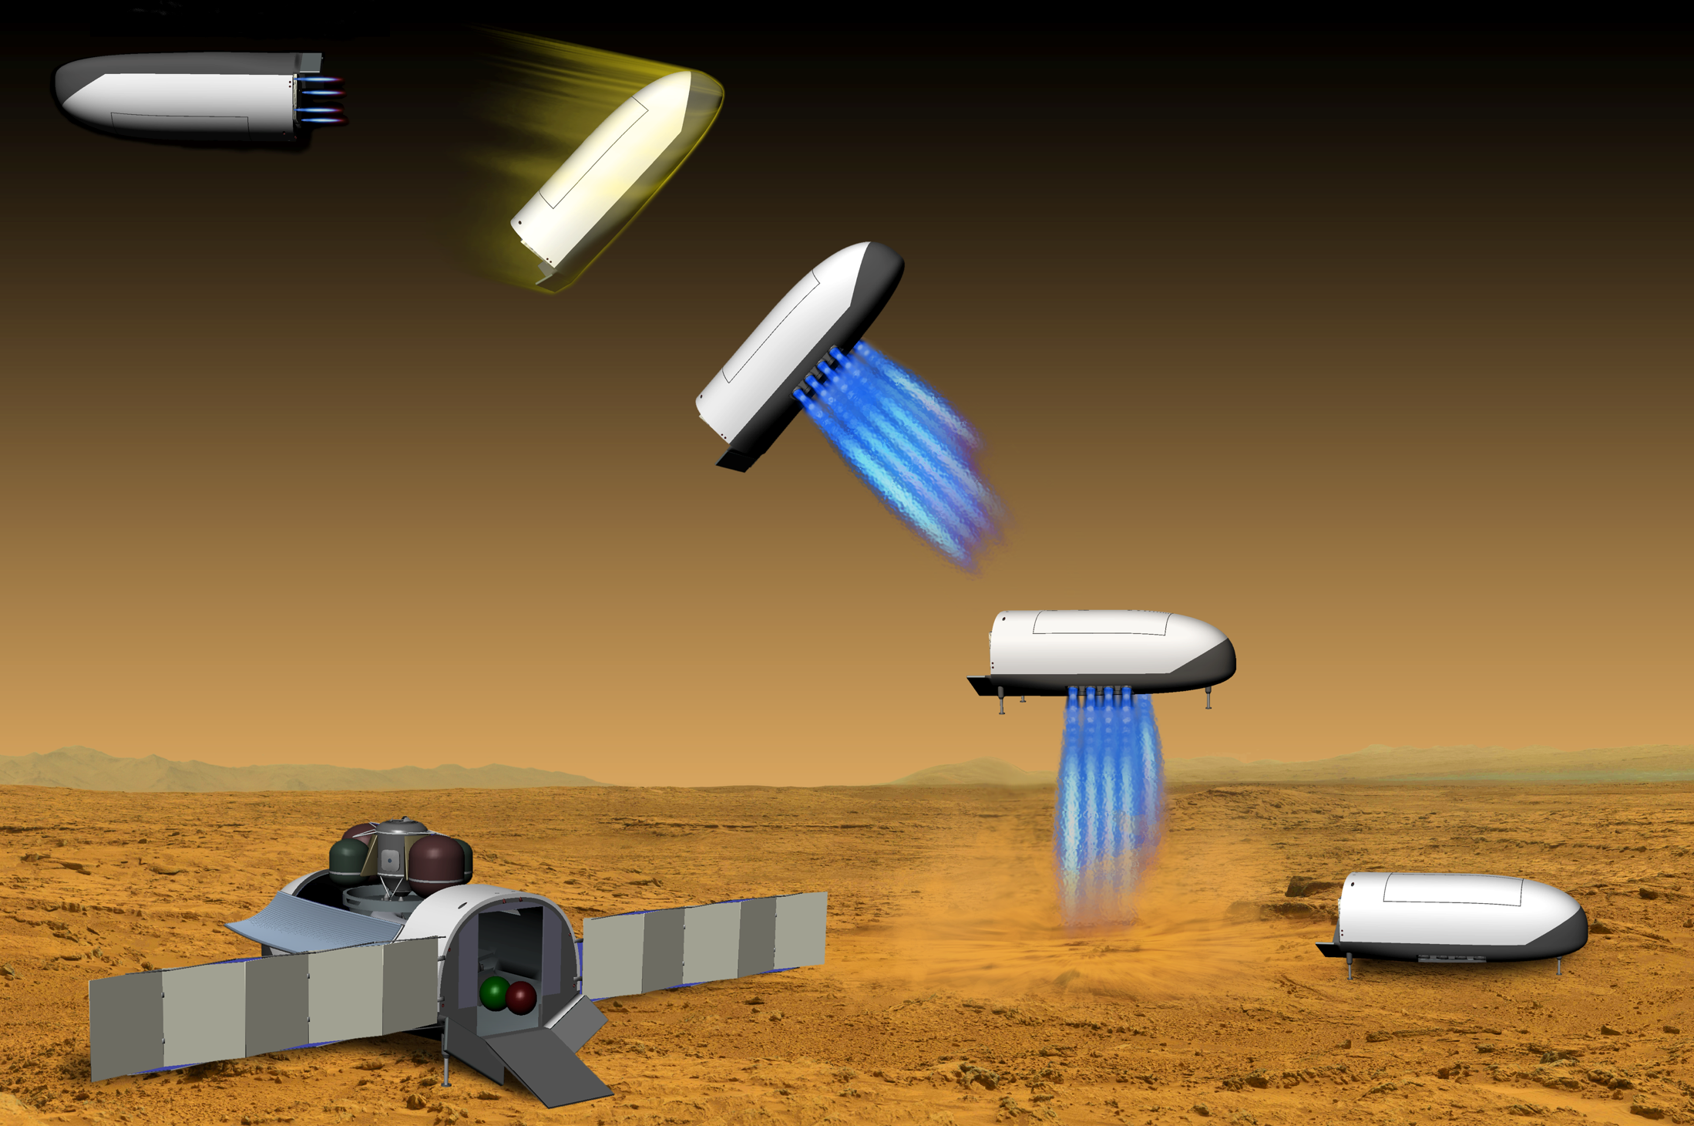
\includegraphics[width=\linewidth]{Figures/CobraMRV.png}
		\caption{CobraMRV Design. Source: C. Cerimele et al. A rigid mid lift-to-drag ratio approach to human mars entry, descent,
			and landing. AIAA Paper, 2017-1898, 2017. \label{fig:CobraMRV} }
	\end{minipage}
\end{figure}

In their paper, Cerimele et. al 2017\:\cite{CERIMELE} provide maximum thrust $T_{max}$ as well as mass, lift and drag characteristics, and other factors important for physical modeling and simulation to be described in more detail in Section\:\ref{chap:simulation}. The maximum thrust magnitude $T_{max}$ is given as $800\:kN$, and the vehicle's mass as the start of powered descent initiation is $58,000 kg$. 

\chapter{METHODOLOGY} \label{chap:methodology}
To investigate a guidance law with careful focus on the time-to-go approach, a law must be developed and implemented in a simulation framework. The derivation of E-Guidance is presented here in the context of optimal control, as is the time-to-go approach. The derivation of APDG is also presented without claim of optimality.

%In this chapter we see how equations, theorems, figures and tables are
%created, enumerated and referenced.  We also play around with lengths
%of chapter and section headings.  For example, this chapter begins
%with a long chapter heading that must conform to the thesis manual.
%Later on there is a very long section heading.  These examples show
%how the sdsu thesis class file automatically handles formating.
\section{Notation}
This paper uses a set of standard mathematical notation in deriving algorithms and describing models. That notation is defined here.

Vectors consisting of three coordinates in the guidance frame are indicated by bold face type as in Equation\:(\ref{eqn:vectordef}). Also relevant in this equation is that vectors are defined as column matrices.

\begin{equation}
\label{eqn:vectordef}
\bm{V} = 
\begin{bmatrix}
V_1 \\
V_2 \\
V_3
\end{bmatrix}
\end{equation}

Matrices are represented by capital letters as in Equation\:(\ref{eqn:matrixdef}). All matrices in this paper are 3x3 matrices.

\begin{equation}
\label{eqn:matrixdef}
A = 
\begin{bmatrix}
	a_1 & a_2 & a_3 \\
	a_4 & a_5 & a_6 \\
	a_7 & a_8 & a_9
\end{bmatrix}
\end{equation}

A column vector $\bm{V}$ may be converted to a row vector via a transpose operation.

\begin{equation*}
\bm{V}^T = [V_1\:\:V_2\:\:V_3]
\end{equation*}

Vector multiplication arises mainly in three ways, all used throughout the guidance algorithm derivation. The first is the vector dot product, indicated as in Equation\:(\ref{eqn:dotdef}).

\begin{equation}
\label{eqn:dotdef}
\bm{a}\cdot\bm{b} = \bm{a}^T\bm{b} = a_1b_1 + a_2b_2 + a_3b_3
\end{equation}

Vectors consist of a magnitude and a direction. The magnitude is calculated by way of a vector norm operation as in Equation\:(\ref{eqn:normdef})

\begin{equation}
\label{eqn:normdef}
||\bm{V}|| = \sqrt{\bm{V}^T\bm{V}}
\end{equation}

The direction of a vector is itself a vector of magnitude 1 which points in the direction of the vector. A direction vector is indicated by a hat $\hat{\bm{g}}$ as in Equation\:(\ref{eqn:hatdef}). This equation represents the direction of gravitational acceleration as a function of position $\bm{r}$.

\begin{equation}
\label{eqn:hatdef}
\hat{\bm{g}} = \frac{\bm{g(\bm{r})}}{||\bm{g(\bm{r})}||}
\end{equation}


The second vector multiplication operation is the cross product of two vectors, indicated by $\times$ as in Equation\:(\ref{eqn:crossdef}) for two vectors $\bm{a}$ and $\bm{b}$ in frame $\hat{\bm{e}}$, where $|A|$ represents the determinant of matrix $A$. 

\begin{equation}
\label{eqn:crossdef}
\bm{a}\times\bm{b} = 
\left|
\begin{matrix}
\hat{\bm{e_1}} & \hat{\bm{e_2}} & \hat{\bm{e_3}} \\
a_1 & a_2 & a_3 \\
b_1 & b_2 & b_3
\end{matrix}
\right|
\end{equation}


The third vector multiplication operation is left matrix multiplication as in Equation\:(\ref{eqn:matrixmultdef}). As shown, left matrix multiplication of a 3x3 matrix $A$ with a 3x1 vector $\bm{x}$ results in a 3x1 vector $\bm{b}$. 

\begin{equation}
\label{eqn:matrixmultdef}
A\bm{x} = \bm{b} =
\begin{bmatrix}
b_1 \\
b_2 \\
b_3
\end{bmatrix}
\end{equation}

Equation\:(\ref{eqn:matrixmultdef}) can be interpreted as a system of linear equations in 3 unknowns: $x_1$, $x_2$, and $x_3$. The solution to this linear system requires evaluations of the inverse of the matrix $A$, represented by $A^{-1}$. 

Time derivatives are represented with dot notation as in Equation\:(\ref{eqn:timedotdef}) showing the derivative relationship between position and velocity vectors.

\begin{equation}
\label{eqn:timedotdef}
\frac{d\bm{r}}{dt} = \dot{\bm{r}} = \bm{V}
\end{equation}


\section{Coordinate Frame}
The guidance algorithm is developed within the guidance coordinate frame $\bm{\hat{e}}$. This frame can be defined in several ways. Cherry\:\cite{CHERRY} used a gravitational body-centered frame to develop E-Guidance, but any inertial frame can be appropriate. The simulation uses a body-centered frame such that Initial and Final conditions are defined by longitudes, latitudes, and radii from the center of Mars. This simulation neglects the body rotation, but it could be taken into account by defining a rotated final landing site and would not alter the problem qualitatively. 

For convenience these Initial Conditions are presented in Table\:\ref{tab:IC} after a coordinate transformation to a frame centered on the landing cite so that the final position constraint\:(\ref{eqn:constraint_r}) is at the origin. This frame is a right-handed system such that the first coordinate is Mars East, the second is Mars North, and the third is Mars up (the direction opposite the local gravitational acceleration, $-\hat{\bm{g}}$). This E-N-U frame is intuitive because mission conditions such as ground range and altitude are directly represented.  


\section{Guidance Law} \label{sec:guidancelaw}
The guidance law under investigation is Apollo Powered Descent Guidance (APDG), first presented in Cherry\:1964\:\cite{CHERRY}. APDG is a version of E-Guidance, which was developed empirically by integrating the equations of motion and choosing basis functions for the total acceleration $\bm{a}$ that provided the necessary degrees of freedom to satisfy the terminal constraints in Equations\:(\ref{eqn:constraint_r}) and\:(\ref{eqn:constraint_V}). With control over thrust acceleration (and therefore total acceleration), satisfying the initial conditions after integration of the equations of motion requires two basis functions with vector coefficients. APDG extends this approach to controlled final attitude by adding an additional constraint on final thrust acceleration $\bm{a}^*_{T_f}$ as in Equation\:(\ref{eqn:constraint_a}), and satisfying these three vector constraints requires a further third basis function. 

Guidance laws are typically presented as functions or systems defined over a range of time-to-go $t_{go} \epsilon [t_{go_0}, 0)$. If the guidance command were recomputed without updated state information in nominal conditions and with an extremely accurate physical model the vehicle would satisfy the terminal constraints without issue. However, in the presence of measurement error this open-loop strategy, which does not feed back the current state, will fail. Instead, these guidance laws can be recomputed at each update treating the current vehicle state as the initial condition for the guidance problem to be solved. In this was the state feedback results in a closed-loop formulation that is robust and can much more accurately satisfy constraints in real world applications. Good guidance law formulations result in arbitrary initial conditions such that the law can be implemented in a closed-loop fashion.

The derivation of E-Guidance as developed by Cherry proceeds below, followed by its formulation as an optimal guidance problem. APDG is then derived as developed by Cherry in a similar fashion though no claim is made about its optimality. The relative performance of the two laws is examined in Chapter\:\ref{chap:results}.

%
%You can have fun formulas, such as $x= 7 y^x$.  If you want the
%equations displayed you can use two dollar signs, \$\$ to enclose the
%mathematics, or you can use
%
%\medskip\noindent
%\texttt{%
%  \hspace*{2em}$\backslash$begin\{equation*\} \\
%  \hspace*{3em}math stuff \\
%  \hspace*{2em}$\backslash$end\{equation*\}
%}\\%
%as in
%
%\medskip\noindent\hspace*{2em}\begin{minipage}{4.5in}
%\begin{verbatim}
%\begin{equation*}
%  \int_{\partial \Omega} \omega = \int_{\Omega} d\omega.
%\end{equation*}
%\end{verbatim}
%\end{minipage}
%
%\medskip\noindent
%which produces
%\begin{equation*}
%  \int_{\partial \Omega} \omega = \int_{\Omega} d\omega.
%\end{equation*}
%
%There are several other ways to display equations.  The code for this
%one (which you can see in \verb+body.tex+) aligns all the equal
%signs.
%\begin{align}
%  (x+2)^3 & = (x+2)(x+2)^2 \\
%  &= (x+2)(x^2+4x+ 4) \\
%  &= x^3+ 6x^2 + 12*x + 8
%\end{align}
%Notice that this last set of equations is numbered, but the previous
%one is not.  The * in the \LaTeX\ code eliminates the numbering.
%

%\section{Equations}
%
%Enumeration of equations, theorems, definitions, tables, is handled
%automatically by \LaTeX.  Each of these items may be given a label
%using \verb+\label{<labelname>}+.  The item can then be refered to
%by \verb+\ref{<labelname>}+.  Below we demonstrate how
%to create and label an equation. Our first is a general differential
%equation,
%\begin{equation}
%  \dot{x} = f(t,x),\qquad x(0)= x_0. \label{de1}
%\end{equation}
%To see that the numbering is going fine we insert a matrix system as
%follows:
%\begin{equation}
%  \dot{y} =
%  \begin{bmatrix}
%    a_1 & 0 & \cdots & 0 \\
%    0 & a_2 & \cdots & 0 \\
%    \vdots & \vdots & \ddots & \vdots \\
%    0 & 0 & \cdots & a_n
%  \end{bmatrix}
%  y.
%  \label{de2}
%\end{equation}
%The numbering is valuable when one wants to refer to the
%Equations~(\ref{de1}) and\:(\ref{de2}). Note that when referring to
%Equation~(\ref{de1}) you must capitalize the word equation. Also, when
%you enter a specific equation, figure, or table, \emph{e.g.,}
%Eqn.~(\ref{de1}), then you should type a $\tilde{\phantom{x}}$ between
%the word Eqn., Fig., or Table and its labeling number to prevent
%inappropriate division of the label at the end of a line.
%
%To display an equation without numbering, one uses the math
%displaystyle mode which works as follows:
%\begin{equation*}
%  \dot{y} = g(y),
%\end{equation*}
%which is an autonomous equation in $y$. The $y$ at the end of the last
%sentence is in standard math mode. Further information on equations is
%provided in Appendix~A.
%
%
%\section{Theorems, etc.}
%
%The student needs to highlight important results such as theorems,
%hypotheses, or definitions. In this section we investigate how
%\LaTeX\ handles definitions, theorems, corollaries, etc.
%\begin{definition}   
%  A linear differential equation is asymptotically stable if and only
%  if all eigenvalues, $\lambda$, of the operator matrix have negative
%  real part.
%\end{definition}
%We follow this with a couple of theorems and a corollary.
%\begin{theorem}
%  If the matrix $A$ in the linear differential equation,
%  \begin{equation}
%    \dot{y} = Ay, \qquad y(0) = y_0, \label{lde}
%  \end{equation}
%  is symmetric, then the solution of {\rm\:(\ref{lde})} is
%  non-oscillatory.
%\end{theorem}
%\begin{corollary}
%  If the matrix $A$ in {\rm\:(\ref{lde})} is symmetric and has negative
%  eigenvalues, then the solution is non-oscillatory and asymptotically
%  stable.
%\end{corollary}
%
%In order to check how the numbering proceeds we insert here another
%theorem.
%\begin{theorem}
%  If the matrix $H$ in the linear differential equation,
%  \begin{equation}
%    \dot{y} = Hy, \qquad y(0) = y_0, \label{ldeh}
%  \end{equation}
%  is antisymmetric, then the solution of {\rm\:(\ref{ldeh})} is oscillatory.
%\end{theorem}
%
%The \texttt{thesis.tex} also defines environments for \texttt{lemma}
%and \texttt{proposition} though you can add more if you wish.  For
%example sometimes it is useful to add an \texttt{example} style
%environment.  See the preamble of the document for more information.
%
%
%
%
%











\subsection{Equations of Motion}\label{sec:EOMS}
Derivation of a powered descent guidance law begins with a formulation of the State Equation\:(\ref{eqn:state_equation})
\begin{equation}
\dot{\bm{x}} = \bm{f}(\bm{x,\bm{u}})
\label{eqn:state_equation}
\end{equation}

Cherry derives E-Guidance by treating this set of differential equations as a boundary value problem with initial conditions and final conditions to be satisfied by some command $\bm{u}$. Aerodynamic effects are not considered for development of the law, though they will be simulated and investigated with regards to performance.

The state equations for the 3-dimensional boundary value problem are as follows

\begin{align}
\label{eqn:EoM1}
\bm{\dot{r}} &= \bm{V}                               & \bm{r(t_0)} &= \bm{r_0}\\
\label{eqn:EoM2}
\bm{\dot{V}} &= \bm{g(r)} + \bm{a_T}                           & \bm{V(t_0)} &= \bm{V_0}
\end{align}

%Where 
%\begin{align*}
%\dot{m} &= -\frac{T}{g_0 I_{sp}} & m(t_0) &= m_0\\
%a &= \frac{T}{m(t)} \\
%\end{align*}

with terminal constraints at a fixed final time $t_f$
\begin{align}
\label{eqn:constraint_r}
\bm{r}(t_f) &= \bm{r}^*_f\\
\label{eqn:constraint_V}
\bm{V}(t_f) &= \bm{V}^*_f 
\end{align}

where $\bm{a}_T$ is the thrust acceleration vector and $\bm{g}(\bm{r})$ is gravitational acceleration

\begin{equation}
\label{eqn:gravity}
\bm{g} = -\frac{\mu \bm{r}}{(\bm{r}^T\bm{r})^{(3/2)}}
\end{equation}

where $\mu$ is the standard gravitational parameter for the body in question. For Mars, $\mu \approx 4.282*10^{13}$

Cherry recognized that a desired performance index would minimize the integral of the thrust acceleration magnitude as in Equation\:(\ref{eqn:fueloptimalindex}. He also recognized that the thrust acceleration $\bm{a}_T$ is limited such that

\begin{equation} 
\label{eqn:thrustlimit}
0 < a_{min} \leq ||\bm{a}_T|| \leq a_{max}
\end{equation}

By choosing the command $\bm{u} = \bm{g(r)} + \bm{a}_T$, the thrust acceleration command becomes $\bm{a}_T = \bm{u} - \bm{g(r)}$ so that the nonlinearities of the gravitational acceleration are effectively removed and a boundary value problem can be constructed by directly integrating the equations of motion and applying the boundary values to form a set of linear equations to be solved.

\subsection{E-Guidance}
While the set of non-linear equations presented in Section\:\ref{sec:EOMS} do uniquely define a guidance command $\bm{u}$, Cherry recognized that they represented a ``formidable bunch" of equations that he could not practically solve. Instead, he considered the infinite-dimensional generalized Fourier series that must represent the guidance command $\bm{u}$. By reducing the order of the Fourier series to equal the degrees of freedom demanded by the vector constraints of Equations\:(\ref{eqn:constraint_r}) and\:(\ref{eqn:constraint_a}), Cherry developed E-Guidance by considering first one guidance axis at a time, a ``divide and conquer" strategy, so the acceleration command took the form of Equation\:(\ref{eqn:Cherryaccel}), where $p_1(t)$ and $p_2(t)$ are linearly independent functions of time.

\begin{equation}
\label{eqn:Cherryaccel}
\ddot{x} = c_1p_1(t) + c_2p_2(t)
\end{equation}

Cherry sets $p_1(t) = 1$ and $p_2(t) = t$, mostly for simplicity while recognizing that it may be suboptimal, arriving at a form identical to the one presented in Equation\:(\ref{eqn:command}). 

Cherry also proposes a time-to-go algorithm similar to that in Algorithm\:(\ref{eqn:FPI}). It does not, however, do much to consider the optimality of this algorithm or, more critically, to deal with the problem of powered descent initiation.

\subsection{Optimality} \label{sec:optimality}
Cherry's solution for E-Guidance matches the result from the solution to an optimal guidance problem with a particular performance index.

\subsubsection{Performance Index}
Fuel consumption is related to the thrust acceleration vector by engine parameters represented by some positive constant k

\begin{equation}
\label{eqn:fuel_rate}
\dot{m} = -k ||\bm{a}_T||
\end{equation}

A fuel optimal guidance law should therefore use the performance index
\begin{equation}
\label{eqn:fueloptimalindex}
J = \int_{t_0}^{t_f} ||\bm{a}_T||dt
\end{equation}

Choosing to minimize the square of the total acceleration $\bm{a} = \bm{g} + \bm{a}_T$ gives a performance index
\begin{equation}
\label{eqn:performanceindex}
J = \frac{1}{2} \int_{t_0}^{t_f} (\bm{g}+\bm{a}_T)^T(\bm{g}+\bm{a}_T)dt
\end{equation}

For a constant gravitational acceleration $\bm{g}$, this performance index attempts to minimize $||\bm{a}_T||^2$. It is not fuel optimal as in Equation\:(\ref{eqn:fueloptimalindex}), but it does provide a cost to large thrust accelerations and might be expected to give good fuel performance.

\subsubsection{E-Guidance As An Optimal Guidance Law}
Choosing the guidance command $\bm{u} = \bm{g} + \bm{a}_T$ and applying optimal control theory results in the Hamiltonian in Equation\:(\ref{eqn:Hamiltonian}) to be maximized and the steps following to define the behavior of the command $\bm{u}$.

\begin{equation}
\label{eqn:Hamiltonian}
H = \bm{p}_r^T\bm{V} + \bm{p}_V^T\bm{u} - \frac{1}{2}\bm{u}^T\bm{u}
\end{equation}

\begin{equation*}
\dot{\bm{p}}_r = -\frac{\partial H}{\partial \bm{r}} = 0 \implies \bm{p}_r = -\bm{c}_2
\end{equation*}
\begin{equation*}
\dot{\bm{p}}_V = -\frac{\partial H}{\partial \bm{V}} = -\bm{p}_r \implies \bm{p}_V = \bm{c}_1 + \bm{c}_2 t
\end{equation*}
\begin{equation*}
\frac{\partial H}{\partial \bm{u}} = 0 \implies \bm{u} = \bm{p}_V = \bm{c}_1 + \bm{c}_2 t
\end{equation*}

For convenience, let $\tau = t_f - t$
\begin{equation}
\label{eqn:command}
\bm{u} = \bm{k}_1 + \bm{k}_2 \tau
\end{equation}
where $\bm{k}_1$ and $\bm{k}_2$ are constant vectors.

Integrating the equations of motion with $\bm{\dot{V}} = \bm{u}$ then gives
\begin{equation}
\label{eqn:EoM_solve_1}
\int\bm{\dot{V}}(t) dt  = \bm{k}_1(t-t_0) + \frac{1}{2}\bm{k}_2(t-t_0)^2 + \bm{V}(t_0) 
\end{equation}

\begin{equation}
\int \bm{\dot{r}}(t)dt = \frac{1}{2} \bm{k}_1(t-t_0)^2 + \frac{1}{6}\bm{k}_2(t-t_0)^3 + \bm{V}(t_0)(t-t_0) + \bm{r}(t_0) 
\label{eqn:EoM_solve_2}
\end{equation}

Setting $t = t_f$ and letting $t_{go} = t_f - t_0$ satisfies the terminal constraints from Equations\:(\ref{eqn:constraint_r}) and\:(\ref{eqn:constraint_V}), resulting in 6 linear equations in 6 unknowns

\begin{align}
\label{eqn:system1}
\bm{k}_1 t_{go} + \frac{1}{2}\bm{k}_2 t_{go}^2 &= \bm{V}_f^* - \bm{V}_0\\
\label{eqn:system2}
\frac{1}{2}\bm{k}_1 t_{go}^2 + \frac{1}{6}\bm{k}_2 t_{go}^3 &= \bm{r}_f^* - \bm{r}_0 - \bm{V}_0t_{go}
\end{align}

These equations can be separated into sets of two per vector component. Define an inertial guidance frame $\bm{e} = (\hat{x},\hat{y},\hat{z})^T$ such that guidance vector $\bm{u}$ is composed of components in $\bm{e}$, $\bm{u} = (u_{x},u_{y},u_{z})^T$. For the equations in $\hat{x}$ we have

\begin{equation}
  \label{eqn:E_system}
  \begin{bmatrix}
    t_{go} & \frac{1}{2}t_{go}^2 \\
    \frac{1}{2}t_{go}^2 & \frac{1}{6}t_{go}^3 \\
  \end{bmatrix}
 \left(
	\begin{matrix}
	k_{1_x} \\ 
	k_{2_x} 
	\end{matrix}
\right) = 
 \left(
	\begin{matrix}
	V_{f_x}^* - V_{0_x} \\ 
	r_{f_x}^* - (r_{0_x} + V_{0_x}t_{go}) 
	\end{matrix}
\right)
\end{equation}

Solving the two-equation system is accomplished by inverting the left-hand matrix, leading to a coefficient matrix $E$
\begin{equation}
E = 
	\begin{bmatrix}
	-2/t_{go} & 6/t_{go}^2 \\
	6/t_{go}^2 & -12/t_{go}^3
	\end{bmatrix}
\end{equation}

The coefficients in $\hat{x}$ are then
\begin{equation}
\label{eqn:simplelaw}
\begin{pmatrix}
k_{1_x} \\
k_{2_x}
\end{pmatrix}
= E
\begin{pmatrix}
V_{f_x}^* - V_{0_x} \\ 
r_{f_x}^* - (r_{0_x} + V_{0_x}t_{go}) 
\end{pmatrix}
\end{equation}

It can be shown that the equations in $\hat{y}$ and $\hat{z}$ take the same form. This $2x2$ $E$ matrix is the origin of the name \textit{E-Guidance}, the guidance law used in the Apollo lunar landing missions.

\subsection{Apollo Powered Descent Guidance} \label{sec:APDG}

APDG enforces a final attitude constraint as a matter of practicality. A real rocket landing would typically require that the vehicle be oriented in a specific direction upon landing. Without explicitly enforcing a final attitude, the vehicle could touch down at a large angle while still satisfying final velocity and position constraints. For a vehicle whose attitude is determined by the thrust acceleration vector, this constraint can be implemented as a final thrust acceleration constraint as in Equation\:(\ref{eqn:constraint_a}).

\begin{equation}
\label{eqn:constraint_a}
\bm{a}_T(t_f) = \bm{a}^*_{T_f}
\end{equation}

A logical choice for this final thrust acceleration constraint is a vector in the negative gravitational acceleration direction as in Equation\:(\ref{eqn:constraint_ag}) where c is some positive scalar, ensuring that the vehicle touches down vertically. 

\begin{equation}
\label{eqn:constraint_ag}
\bm{a}^*_{T_f} = -c\bm{\hat{g}}
\end{equation}

This vector constraint cannot be satisfied with only two basis functions for the command $\bm{u}$, so a third linearly independent function must be introduced such that $\bm{u} = \bm{c}_1 p_1(t) +\bm{c}_2 p_2(t) + \bm{c}_3 p_3(t)$. Cherry's choice for the third basis function is $p_3(t) = t^2$ for simplicity, with the other two functions the same as in E-Guidance.

After applying the substitution from Equation\:(\ref{eqn:command}), this choice gives a command $\bm{u} = \bm{k}_1+\bm{k}_2 \tau + \bm{k}_3 \tau^2$. This form for the command input is also easily integrable and leads to a similar linear system of 9 equations in $\bm{k_1}$, $\bm{k_2}$, and $\bm{k_3}$. Using the same guidance frame $\hat{e}$ defined for Equation\:(\ref{eqn:E_system}) and considering one coordinate at a time we get a system similar to E-Guidance in Equation\:(\ref{eqn:APDGlaw})

\begin{equation}
\label{eqn:APDGlaw}
\begin{pmatrix}
k_{1_x} \\
k_{2_x} \\
k_{3_x}
\end{pmatrix}
= 
\begin{bmatrix}
0 & 0 & 1 \\
18/t_{go}^2 & -24/t_{go}^3 & -6/t_{go}\\
-24/t_{go}^3 & 36/t_{go}^4 & 6/t_{go}^2
\end{bmatrix}
\begin{pmatrix}
V_{f_x}^* - V_{0_x} \\ 
r_{f_x}^* - (r_{0_x} + V_{0_x}t_{go}) \\
g_x + a_{f_x}^*
\end{pmatrix}
\end{equation}


\subsection{Time-to-go} \label{sec:Time-to-go}
APDG depends upon a reliable estimate of remaining time-to-go ($t_{go}$). The Apollo mission's guidance used an estimate that updated continuously using Newton's method, but it was intended to only operate until start of the terminal descent phase at which point guidance switched to a manual vertical descent operation. Updating the $t_{go}$ estimate continuously is attractive since it should be robust; if conditions have to change during the mission a closed-loop (continuously updating) solution will adjust and a new, realistic $t_{go}$ will feed into the guidance solution. This quality was important to the Apollo Guidance solution because it relied upon pilot inputs to define the landing location visually, which meant allowing for landing site redesignations mid-mission. If $t_{go}$ was not recomputed after site redesignation, the guidance law would command unrealizable thrust acceleration commands.

For the purposes of this study, live landing site redesignation was not considered. Without the possibility of landing site redesignation, an open-loop $t_{go}$ solution lends the guidance law more stability in that the performance is less dependent upon specific assumptions and conditions imposed by the $t_{go}$ algorithm. For instance, one closed-loop $t_{go}$ algorithm is implemented in Algorithm\:(\ref{eqn:FPI}).

\begin{algorithm}
	\caption{Fixed-Point-Iteration $t_{go}$}\label{eqn:FPI}
	\begin{algorithmic}[1]
		\State $tol\gets c$
		\While{$|t_{go_0} - t_{go_1}| \geq tol$}
		\State $t_{go_0} \gets t_{go_1}$
		\State $\Delta V \gets \sqrt{(\bm{V}-\bm{V_0} + \bm{g}\cdot t_{go})^T(\bm{V}-\bm{V_0} + \bm{g}\cdot t_{go_0})}$
		\State $t_{go_1} \gets \frac{m_0}{\dot{m}}\left(e^{\frac{-\Delta V}{v_{ex}}}-1\right)$ \Comment{$\dot{m} < 0$}
		\EndWhile
		\State \textbf{return} $t_{go_1}$
	\end{algorithmic}
\end{algorithm}

Each guidance update uses the previous update's $t_{go}$ minus clock time as its initial guess $t_{go_0}$, and the max iterations may be limited to some reasonable number.

This algorithm requires an assumption about a fixed mass flow rate $\dot{m}$ which is not guaranteed by the guidance law. Adjustment of this mass flow rate estimate is very particular to the initial conditions of the mission, resulting in a necessarily conservative $t_{go}$ to account for initial condition dispersion.

One attractive open-loop option is the time to perform a gravity turn landing at maximum thrust. Equation\:(\ref{eqn:tgoGT}) for a gravity turn time-to-go, $t_{go_{GT}}$, was presented in Citron, Dunin, and Meissinger 1964\:\cite{CITRON}. After engine ignition and initiation of Powered Descent Guidance, the updated time-to-go is computed as $t_{go_{GT}}$ minus elapsed clock time. The algorithm for time-to-go using a gravity turn maneuver is given in Equation\:(\ref{eqn:tgoGT}), where $a_{GT}$ is the thrust acceleration magnitude applied during the maneuver. This equation gives two roots for $a_{GT}$, a positive root and a negative root. The desired root is positive, making it a simple matter to find. This quantity will be important in section\:\ref{sec:PDI}.

\begin{align}
\label{eqn:tgoGT}
\begin{split}
\gamma &= \frac{\pi}{2} - cos^{-1}\left(\frac{\bm{r}^T\bm{V}}{||\bm{r}||||\bm{V} ||} \right) \\
g_m &= ||\bm{g}|| \\
r_m &= ||\bm{r}|| \\
V_m &= ||\bm{V}|| \\
a &= 1/g_m^2 \\
b &= \frac{sin(\gamma)V_m^2}{2(r_m-R_M)g_m^2} \\
c &= -\frac{V_m^2 (1+sin(\gamma)^2)}{4(r_m - R_M)g_m}+1 \\
a_{GT} &= \frac{-b \pm \sqrt{b^2 - 4 a c}}{2 a} \\
t_{go_{GT}} &= \frac{V_m}{2} \left(\frac{1+sin(\gamma)}{a_{GT} + g_m} + \frac{1-sin(\gamma)}{a_{GT} - g_m} \right)
\end{split}
\end{align}

A gravity turn landing does not directly apply to the general powered descent guidance problem under investigation because it does not seek to satisfy the constraints given in Equations\:(\ref{eqn:constraint_r}) and\:(\ref{eqn:constraint_V}). However, if the magnitude of the terminal velocity target in Equation\:(\ref{eqn:constraint_V}) is small, the required time to decelerate from an initial $\bm{V}_0$ under only the forces of thrust acceleration $\bm{a}_T$ and gravity $\bm{g}$ is, at minimum, the gravity turn solution $t_{go_{GT}}$. Since the terminal position $\bm{r}_f$ is specified, the vehicle necessarily needs more time than given by the gravity turn solution to satisfy it. Assuming a small trajectory error requiring a small diversion to landing site, a small constant factor $ c_t \approxeq 1.2$ can be applied to the gravity turn time-to-go to allow for redirection. The choice of $c_t = 1.2$ will prove to be sufficiently conservative to survive initial condition dispersion, rocket parameter dispersion, and navigation error. 

\section{Adaptive Powered Descent Initiation} \label{sec:PDI}
The central focus of this thesis is the use of Adaptive Powered Descent Initiation (PDI) to improve the fuel performance of APDG. This is accomplished by choosing an ignition time which results in superior propellant consumption. From Leitmann's\:\cite{LEITMANN} and Meditch's\:\cite{MEDITCH} work it is expected that a ``bang-bang" style thrust profile is desirable. Lu 2017 \:\cite{LU} shows that for the three-dimensional problem the propellant optimal thrust profile is indeed ``bang-bang" style and may have up to two switches. He also shows that the profile is further constrained to a final thrust value $T(t_f) = T_{max}$ in order to satisfy the final position and velocity constraints. With APDG controlling the thrust acceleration vector $\bm{a}_T$, a ``bang-bang" style thrust profile will not be realized due to the continuous nature of the boundary-value problem presented, but the ignition time may be chosen to force a thrust profile closer to optimum. By choosing a time-to-go carefully, nearly optimal fuel performance may be expected. 

Since APDG does not take the thrust acceleration limits of Equation\:(\ref{eqn:thrustlimit}) into account directly the time-to-go must do so or risk the required thrust acceleration exceeding the capabilities of the landing vehicle. One approach is to make use of the gravity turn solution as discussed in Section\:\ref{sec:Time-to-go}, Equation\:(\ref{eqn:tgoGT}). This equation provides one criterion for ignition through the specified thrust acceleration $\bm{a}_{GT}$ as in Algorithm\:(\ref{eqn:thrustcriterion}). If the gravity turn time-to-go $t_{go_{GT}}$ is used and the engine ignited for APDG the moment the magnitude of the specified thrust acceleration $a_{GT}$ reaches or exceeds the known maximum thrust acceleration magnitude $a_{max}$, APDG will command a large initial thrust acceleration which may exceed the rocket's limits and the thrust will be nearly or completely saturated at its upper limit. This approaches the optimal ``bang-bang" style thrust profile using minimum thrust ($T = 0$) until ignition and nearly maximum thrust after ignition until landing. Using a padded $t_{go_{GT}}$ helps ensure that there is some margin for error.




\begin{algorithm}[H]
	\caption{Thrust Acceleration Criterion}\label{eqn:thrustcriterion}
	\begin{algorithmic}[1]
		\If {$|\bm{a}_{GT}| \geq \frac{T_{max}}{m}$}
			\State $ ignite\: engine $
		\EndIf
	\end{algorithmic}
\end{algorithm}




Another important criterion is the downrange travel required by a gravity turn maneuver. The powered descent phase should be initiated if the horizontal distance remaining in the velocity direction to the landing site is greater than or equal to the downrange distance traveled during a gravity turn maneuver. This will help ensure that the vehicle does not overshoot the landing site which would ultimately require far more fuel than necessary. Equation\:(\ref{eqn:rangeGT}) gives the downrange distance traveled during a gravity turn maneuver $s_{GT}$, where $h$ is the current altitude. Algorithm\:(\ref{eqn:rangecriterion}) details this ignition logic.

\begin{equation}
\label{eqn:rangeGT}
\begin{split}
s_{GT} = \frac{V_m^2}{2a_{GT})}cos(\gamma)\frac{V_m^2+2g_mh}{V_m^2+g_mh}\frac{R_M}{r_m}
\end{split}
\end{equation}

\begin{algorithm}
	\caption{Range Criterion}
	\label{eqn:rangecriterion}
	\begin{algorithmic}[1]
		\If {$|s_{GT}| \leq |\bm{r}_{xy} - {\bm{r_f}}_{xy}|$}
			\State $ ignite\: engine $
		\EndIf
	\end{algorithmic}
\end{algorithm}

Notably, Cerimele et. al\:\cite{CERIMELE} recognize in the design of the CobraMRV (described in Section\:\ref{sec:CobraMRV}) that ``the selection of the altitude to transition to powered descent ... is a crucial performance variable." They suggest a timing strategy similar to that described in this section.

\chapter{SIMULATION} \label{chap:simulation}

The powered descent simulation (PD Sim) is developed using standard programming techniques and numerical methods. The code is modular to facilitate design and reflect the functions of a mission computer. The simulation has three degrees of freedom (3-DoF) with derived orientation for force modeling. The simulation takes a set of initial conditions $\bm{r}_0$ and $\bm{V}_0$, a set of final conditions $\bm{r}_f$ and $\bm{V}_f$, dispersed rocker parameters, and nominal rocket parameters for the guidance module to use in its calculations of throttle setting.

At the core of the simulation is numerical time integration. The method employed is a 4th order Runge-Kutta (RK4). The RK4 function is called at each time step to progress the simulation forward.

The separate modules called during simulation are the guidance computer which contains the guidance law and computes a commanded thrust acceleration vector, the navigation module which generates a state estimate from simulated instrument measurements for use by the guidance computer, and the aerodynamic module which contains a model of the landing vehicle to compute forces and orientation for use in integration.

The simulation stops when either the vehicle passes through zero altitude (crashes) or the time-to-go is less than a single time integration step. When the latter condition is met, the time integration step is reduced to the remaining time-to-go and one more iteration is performed.

The full simulation code is wrapped in a Monte-Carlo script. The Monte-Carlo script calls the PD Sim with simulation settings, vehicle parameters, initial condition, and navigation uncertainty. This allows each individual run to have dispersed conditions without modification of the code.

Further detail for each part of the simulation follows.

\section{Numerical Integration} \label{sec:RK4}
The numerical time integration is done via a standard Runge-Kutta formulation, presented here as in Ferziger and Peri\'c 2002\:\cite{FERZIGER}. The state vector $\bm{\phi}$ is passed to the equations of motion $\bm{f}(\bm{\phi},t)$ several times as in Equation\:(\ref{eqn:RK4}). $\Delta t$, the time integration step for the simulation, is fixed at 1 millisecond ($10^{-3}$ s). This is shown to be sufficiently small in Section\:\ref{sec:convergence}.

\begin{align}
\label{eqn:RK4}
\begin{split}
\bm{\phi}_{n+\frac{1}{2}}^* &= \bm{\phi}_n + \frac{\Delta t}{2} \bm{f}(t_n,\bm{\phi}_n)\\
\bm{\phi}_{n+\frac{1}{2}}^{**} &= \bm{\phi}^n + \frac{\Delta t}{2}  \bm{f}(t_{n+\frac{1}{2}},\bm{\phi}^*_{n+\frac{1}{2}})\\
\bm{\phi}_{n+1}^* &= \bm{\phi}^n + \Delta t  \bm{f}(t_{n+\frac{1}{2}},\bm{\phi}^{**}_{n+\frac{1}{2}})\\
\bm{\phi}_{n+1} &= \bm{\phi}^n + \frac{\Delta t}{6}
[\bm{f}(t_n,\bm{\phi}_{n})
+ 2\bm{f}(t_{n+\frac{1}{2}},\bm{\phi}^*_{n+\frac{1}{2}})\\
&\:+ 2\bm{f}(t_{n+\frac{1}{2}},\bm{\phi}^{**}_{n+\frac{1}{2}})
+ \bm{f}(t_{n+1},\bm{\phi}_{n+1}^*)]
\end{split}
\end{align}


The EOM function computes the derivative of the state vector $\bm{\phi}$. It is the same as the modeled equations of motion in Equations\:(\ref{eqn:EoM1}) and\:(\ref{eqn:EoM2}) but with an additional force term, $\bm{F}_{LD}$, to represent the aerodynamic forces of Lift and Drag. $\bm{\phi}$ is passed in as a $6x1$ column vector such that $\bm{\phi} = [\bm{r}^T,\bm{V}^T]^T$, and the derivatives are calculated as in Equations\:(\ref{eqn:EoM_sim1}) and\:(\ref{eqn:EoM_sim2}).
\begin{align}
\label{eqn:EoM_sim1}
\bm{\dot{r}} &= \bm{V}\\
\label{eqn:EoM_sim2}
\bm{\dot{V}} &= \bm{g(r)} + \bm{a_T} + \frac{\bm{F}_{LD}}{m}
\end{align}

For simplicity, the vehicle's thrust acceleration response to a guidance command is modeled as zero-lag, i.e. perfect control. It assumes that the vehicle instantly and perfectly responds to the commanded $\bm{a}_T$, so the command from the guidance computer, after being put through a thrust magnitude limiter, is the same as the term in Equation\:(\ref{eqn:EoM_sim2}). This is done to separate the study of Guidance laws from the performance of Control laws, as discussed in Section\:\ref{sec:guidancevcontrol}.

\section{Guidance Computer} \label{sec:guidancecomp}
The guidance computer takes as input the current state as provided by the navigation system, the terminal constraints (final position and velocity in the case of E-Guidance, with final acceleration as well in the case of APDG), nominal vehicle max thrust, current vehicle mass, time-to-go, and selection of guidance law.

The output is a throttle setting as a fraction of the nominal max thrust and a direction for the thrust acceleration $\bm{a}_T$. These values are unlimited at the level of the guidance computer, i.e. the throttle setting can be larger than 1 commanding thrust magnitude greater than $T_{max}$. 

In this implementation, the throttle is limited after being passed out of the guidance computer to reflect the real performance constraint represented by Equation\:(\ref{eqn:thrustlimit}). Since the guidance computer only receives nominal $T_{max}$ upon which to base its throttle setting, the resultant command can be off due to engine performance dispersion.

The guidance command is updated periodically at a rate lower than the simulation rate. Here the guidance is refreshed at 5 Hz. It must also stop updating when $t_{go}$ becomes small due to its presence in the denominator for several entries in the E matrices of Equations\:(\ref{eqn:E_system}) and\:(\ref{eqn:APDGlaw}). For the last half second the thrust acceleration is held constant. This has very little impact on landing precision as demonstrated in the Results chapter, Section\:\ref{sec:naverror}.

The time-to-go computation takes place in the guidance module. The computation method is as described in Section\:\ref{sec:Time-to-go}. A gravity turn estimate is used to initialize the simulation, but it is reset upon ignition based on the current conditions and then allowed to run open-loop until simulation stop. The safety factor applied depends upon conditions. In vacuum, a constant factor $c_t = 1.2$ is necessarily applied to ensure soft landing when using the ignition optimization strategy. With atmospheric conditions the additional factor is unnecessary as is demonstrated in Section\:\ref{sec:atmoperf}.

The guidance solution requires specification of the terminal constraints. In both E-Guidance and APDG, the terminal constraints for position and velocity are specified in the same frame as the initial conditions. For the initial conditions listed in Table\:\ref{tab:IC}, the final position constraint is the origin. The simulation operates in a Mars centered frame in order to simplify gravitational calculations and model a spherical body easily, so the final position constraint seen by the guidance computer is $\bm{r}_f = [0,0,R_M]^T$, where $R_M$ is the radius of Mars. The final velocity is chosen as 1 m/s in the down direction. For APDG the final thrust acceleration is given as Equation\:(\ref{eqn:constraint_ag}), where c is chosen to be 2. This more strongly enforces the final attitude constraint than a smaller scalar without imposing too strong a requirement to the detriment of propellant performance.

\section{Ignition trigger}
Ignition time is determined by checking the two criterion discussed in Section\:\ref{sec:PDI}: required thrust acceleration magnitude $a_{GT}$ and downrange distanced traveled by a gravity turn maneuver $s_{GT}$. The vehicle is started in atmosphere on a trajectory roughly in line with the landing site as shown in Figures\:\ref{fig:trajunpowvacgr} and\:\ref{fig:trajunpowatmo_2}. As the vehicle travels along this trajectory with its engine off, these two criterion are constantly checked. Once either one is satisfied, the engine is ignited and the time-to-go estimate is updated as described in Section\:\ref{sec:guidancecomp}. Implementation of the ignition switch is performed in the simulation script by a simple flag that is checked upon guidance updates.

It is important to be certain that the criteria are met at some point in the flight. This strategy ensures that the ignition trigger is flipped in time as is discussed in Section\:\ref{sec:PDIres}. Figures\:\ref{fig:gtcriteriavac} and\:\ref{fig:gtcriteriaatmo} show that gravity turn required thrust acceleration magnitude monotonically increases throughout the unpowered trajectory, and downrange distance traveled in a gravity turn maneuver decreases faster than the vehicle's range from landing site.

\section{Navigation Module} \label{sec:navmod}
The navigation module is fairly simplistic. It has two functions. 

The first function is to model navigation error in the form of normally distributed noise. The function takes the actual vehicle state $\bm{r}$ and $\bm{V}$, adds noise with a distribution specified in the simulation settings of the Monte Carlo script, and creates $\bm{r}_{nav}$ and $\bm{V}_{nav}$ vectors. The noise distribution is chosen to reflect realistic navigation error as provided by an inertial navigation system per the trade study presented in Moesser\:2010\:\cite{MOESSER}. Typical standard deviations are 1\:m position error and 1/3\:m/s velocity error.

The second function is to filter the noisy navigation measurements to produce a smoother estimate of vehicle state. It does this using a simple low-pass filter as in Equation\:(\ref{eqn:LPF}), where $\alpha$ is a chosen filter constant (here $\alpha = 0.3$), $\bm{x}$ is the current nav output of state, $\bm{x}_{prev}$ is the previous filtered state estimate, and $\bm{x}_{est}$ is the current filtered state estimate. 

\begin{equation}
\label{eqn:LPF}
\bm{x}_{est} = \alpha \bm{x}_{prev} + (1-\alpha) \bm{x}
\end{equation}

A Kalman filter would likely be used on a more sophisticated navigation system for a real aerospace vehicle, but given the simplicity of the navigation error and perfect knowledge of the noise distribution, modeling a Kalman filter would likely provide too good an estimate effectively canceling the effects of simulated navigation error.

\section{Aerodynamic Model}
The Aerodynamic model is comprised of Mars atmosphere data from NASA's Mars-GRAM 2010\:\cite{MARSGRAM}, and the vehicle model was developed by Cerimele et. al\:\cite{CERIMELE}

\subsection{Atmosphere Model}
The atmosphere model is based on NASA's Mars-GRAM 2010\:\cite{MARSGRAM}, an engineering-level atmospheric model of the Martian atmosphere. The model used for this simulation is an empirically developed equation to represent the Martian atmosphere data within the mission's envelope. Mars-GRAM 2010 is based on NASA Ames Mars General Circulation Model for altitudes under 80 km.

For this simulation, the Mars-GRAM data is used to calculate a density $\rho$ and a speed of sound $V_{sound}$, from which Mach number is calculated as $||\bm{V}||/V_{sound}$ and lift and drag are calculated as in Equations\:(\ref{eqn:drag}) and\:(\ref{eqn:lift}), where S is a reference area.

\begin{equation}
\label{eqn:lift}
L = \frac{1}{2} \rho |V|^2 S C_L
\end{equation}

\begin{equation}
\label{eqn:drag}
D = \frac{1}{2} \rho |V|^2 S C_D
\end{equation}

A particular feature of the powered descent phase is the change in drag calculation while the engine is ignited. When the guidance system is operating and the rocket is firing, the drag is modeled as half the value computed when the vehicle is unpowered, i.e. during glide. This is due to the rocket plume's aerodynamics. This change is accomplished in the simulation during the PDI phase by simply dividing the reference area by a factor of 2. 

\subsection{Lift and Drag}
The vehicle aerodynamic model is based on the work of Cerimele\:et\:al\:\cite{CERIMELE}. 

The work of Cerimele er al provides a model of the lift and drag coefficients $C_L$ and $C_D$ based on vehicle Mach number and angle of attack. Vehicle angle of attack is determined directly from the thrust acceleration vector $\bm{a}_T$ and the vehicle velocity vector $\bm{V}$.

Cerimele also provide the reference area S as 62.21 $m^2$. Upon ignition, the vehicle lift and drag is reduced due to the aerodynamic effects of the exhaust plume. This is modeled simply by reducing the reference area to S/2. This effect obviously impacts the fuel performance of APDG, but it does not qualitatively affect the performance of Adaptive PDI as will be clear in Chapter\:\ref{chap:results}.

During the unpowered phase of approach when PDI is being optimized, the vehicle is held at a constant angle of attack of $55^{\circ}$ to achieve maximum drag. 

\subsection{Orientation}
The vehicle's body Euler angles are computed in a 3-2-1 sequence from the body axes. Since the simulation assumes perfect control, the body axes are computed as Equations\:(\ref{eqn:body_Y}),\:(\ref{eqn:body_P}), and\:(\ref{eqn:body_R}). Pitch, yaw, and roll are then calculated as the angles between the body axes and the planet-fixed guidance frame $\hat{\bm{e}}$. Angle of attack is similarly calculated using the body axes and the velocity vector. The CobraMRV's configuration determines that the thrust acceleration vector be in the direction of the vehicle yaw axis.

\begin{equation}
\label{eqn:body_Y}
\bm{body}_Y = \bm{a}_T/||\bm{a}_T||
\end{equation}

\begin{equation}
\label{eqn:body_P}
\bm{body}_P = \frac{\bm{r} \times \bm{body}_Y}{||\bm{r} \times \bm{body}_Y||}
\end{equation}

\begin{equation}
\label{eqn:body_R}
\bm{body}_R = \bm{body}_Y \times \bm{body}_R
\end{equation}

\section{Monte Carlo}
The Monte-Carlo script calls the PD Sim with simulation settings, vehicle parameters, initial condition, and navigation uncertainty. This allows each individual run to have dispersed conditions without modification of the code. The Monte-Carlo script allows choice of initial condition, fixed or dynamic, as well as specification of rocket parameter dispersion, initial condition dispersion in position and velocity, and navigation noise distribution.

The Monte-Carlo script is designed to allow testing of various scenarios and includes initial condition selection among a set of cases. The cases simulated here are points along a trajectory that passes nearly over the landing site, simulating the trajectory resulting from a typical re-entry and aerobraking glide phase. These cases also include initial velocity information that coincides with the vehicle having traveled unpowered along its trajectory. In fixed initial condition mode the user specifies which initial conditions to test, the initial states are dispersed, and the simulations are run from the dispersed starting conditions. In Adaptive PDI mode the Monte-Carlo script automatically chooses the nominal starting condition as the first point along this trajectory. It then disperses the starting point according to dispersion specifications and performs the number of runs specified by the user.

The dispersion factors are chosen to reflect realistic parameter dispersion. Navigation error is modeled using a normal distribution with standard deviations in accordance with Moesser's 2010\:\cite{MOESSER} work as described in Section\:\ref{sec:navmod}. Rocket parameter dispersion is modeled as a uniform distribution of 2\% of the parameter. Equation\:(\ref{eqn:thrustdisp}) shows this calculation for the maximum thrust dispersion, where $T_{max_{nom}}$ is the nominal maximum thrust expected by the guidance computer and $rand$ is a uniformly distributed random number between zero and one.

\begin{equation}
\label{eqn:thrustdisp}
T_{max} = T_{max_{nom}}*(1+0.02*(1-2*rand))
\end{equation}

Each rocket parameter is modeled in this fashion. Only the nominal rocket parameters and dispersed navigation values can be known to the guidance computer, and the modular design allows this distinction to be made easily. The simulation script calls the guidance computer with nominal max thrust and the guidance computer outputs a throttle setting based on that nominal value, but the simulation script applies thrust limits based on the real dispersed values. 

The separation between nominal and dispersed rocket parameters is also important to the PDI strategy, ideally performed within the guidance computer. The PDI required acceleration criterion is implemented as in Algorithm\:(\ref{eqn:thrustcriterion}), but the guidance computer only has the nominal maximum thrust available to it. Similarly, it only has the dispersed navigation values available for the range criterion in Algorithm\:(\ref{eqn:rangecriterion}).

Initial condition values are normally distributed about their nominal values. The dispersion is applied such that three standard deviations in position dispersion is 1000 m from the mean, and three standard deviations in velocity dispersion is 10 m/s from the mean. 

The Monte-Carlo script maintains repeatable randomness for testing. Each of the individual runs starts with a seed to the simulation environment's random number generation algorithm such that re-running the simulation with the same seed will produce precisely identical results. This pseudo-random quality allows investigation of particular runs and helps the software development cycle immensely. The run seeds are stored directly with the run result data in a table so that if later evaluation shows an oddity that should be examined, the run can quickly be replicated.

\section{Initial Condition} \label{sec:IC}
The initial conditions are listed in Table\:\ref{tab:IC}. These are representative of a trajectory of the CobraMRV vehicle on approach after a de-orbit burn and subsequent targeting, from the work of Cerimele\:et\:al\:\cite{CERIMELE}. They are provided in the guidance frame $\hat{\bm{e}}$, which is oriented such that the origin is at the final landing site, $\hat{\bm{e}}_x$ is pointed ``East", $\hat{\bm{e}}_y$ is pointed ``North", and $\hat{\bm{e}}_z$ is pointed ``Up". The simulation itself runs in a Mars-centered Mars-fixed frame. 

\begin{table}[hbt]
	\centering
	\begin{minipage}{3.5in}
		\centering
		\caption{Initial Conditions for Mars Landing\label{tab:IC}.}
		\begin{tabular}{|c||c|c|c|c|c||}    \hline
			State &	Case & $\hat{e}_x$  &  $\hat{e}_y$ & $\hat{e}_z$ & Unit \\ \hline \hline
			$\bm{r}_0$ & 6 & 6079  & -30720 & 8685 & m \\ \hline
			$\bm{V}_0$ & 6 & -121.0  & 644.1 & -64.82 & m/s \\ \hline
			$\bm{r}_0$ & 5 & 5013  & 25170 & 8054 & m \\ \hline
			$\bm{V}_0$ & 5 & -121.1  & 616.5 & -78.57 & m/s \\ \hline
			$\bm{r}_0$ & 4 & 3947  & -19860 & 7305 & m\\ \hline
			$\bm{V}_0$ & 4 & -120.9  & 589.6 & -91.67 & m/s \\ \hline
			$\bm{r}_0$ & 3 & 2887  & -14790 & 6444 & m \\ \hline
			$\bm{V}_0$ & 3 & -120.1  & 563.3 & -103.9 & m/s \\ \hline
			$\bm{r}_0$ & 2 & 2359  & -12,340 & 5973 & m \\ \hline
			$\bm{V}_0$ & 2 & -119.7  & 550.2 & -109.7 & m/s \\ \hline
			$\bm{r}_0$ & 1 & 1832 & -9949 & 5478 & m \\ \hline
			$\bm{V}_0$ & 1 & -119.8 & 537.0 & -115.4 & m/s \\ \hline
		\end{tabular}
	\end{minipage}
\end{table}

These conditions represent an entry trajectory that is slightly off-target for the landing site and requires both powered deceleration to avoid overshoot as well as redirection to correct the angle error. The trajectory traveled from the furthest starting condition (Case 6) unpowered in a vacuum is plotted in Figure\:\ref{fig:trajunpowvac_1} along with the starting positions for Cases 1 through 6 indicated by an X. Similarly, Figure\:\ref{fig:trajunpowatmo_1} shows the trajectory in atmosphere with the vehicle held at optimum angle of attack. Figure\:\ref{fig:trajunpowvacgr} shows the trajectory error in terms of ground range to landing site as the vacuum trajectory passes over the site at around 48 seconds.

\begin{figure}[H]
	\centering
	\begin{minipage}{4.5 in}
		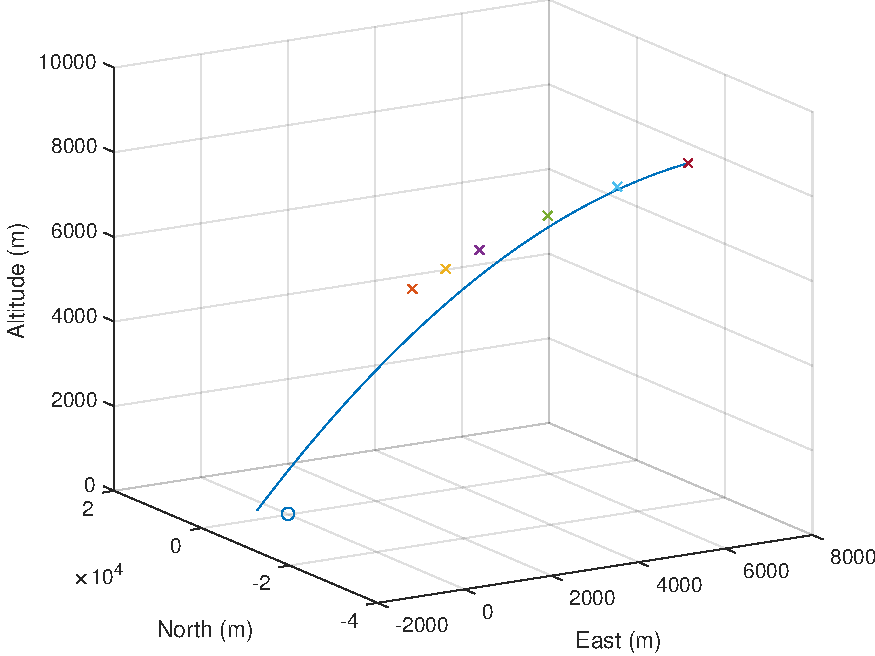
\includegraphics[width=\linewidth]{Figures/trajunpowvac_1.pdf}
		\caption{Unpowered Initial Trajectory in Vacuum \label{fig:trajunpowvac_1} }
	\end{minipage}
\end{figure}

\begin{figure}[H]
	\centering
	\begin{minipage}{4.5 in}
		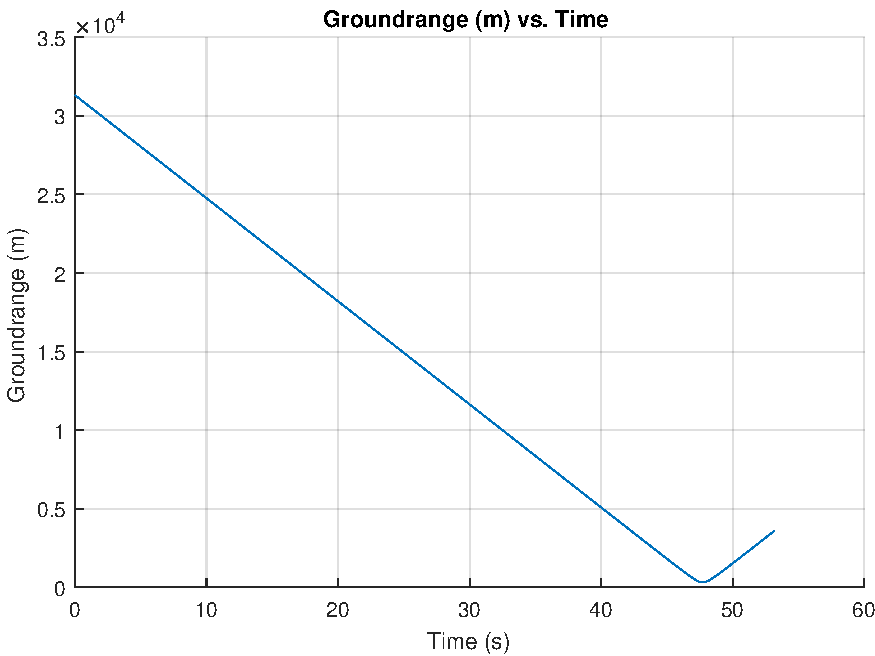
\includegraphics[width=\linewidth]{Figures/trajunpowvacgr.pdf}
		\caption{Ground Range: Unpowered Initial Trajectory In Vacuum \label{fig:trajunpowvacgr} }
	\end{minipage}
\end{figure}

As is clear from Figures\:\ref{fig:trajunpowatmo_1} and\:\:\ref{fig:trajunpowatmo_2} by the placement of the initial conditions of the 6 cases, the initial conditions are chosen to represent the landing vehicle on aerodynamic approach making corrections toward the site. While employing the PDI strategy outlined in Section\:\ref{sec:PDI} the vehicle will travel along the atmospheric trajectory shown in Figures\:\ref{fig:trajunpowatmo_1} and\:\ref{fig:trajunpowatmo_2} until ignition.

\begin{figure}[H]
	\centering
	\begin{minipage}{4.5 in}
		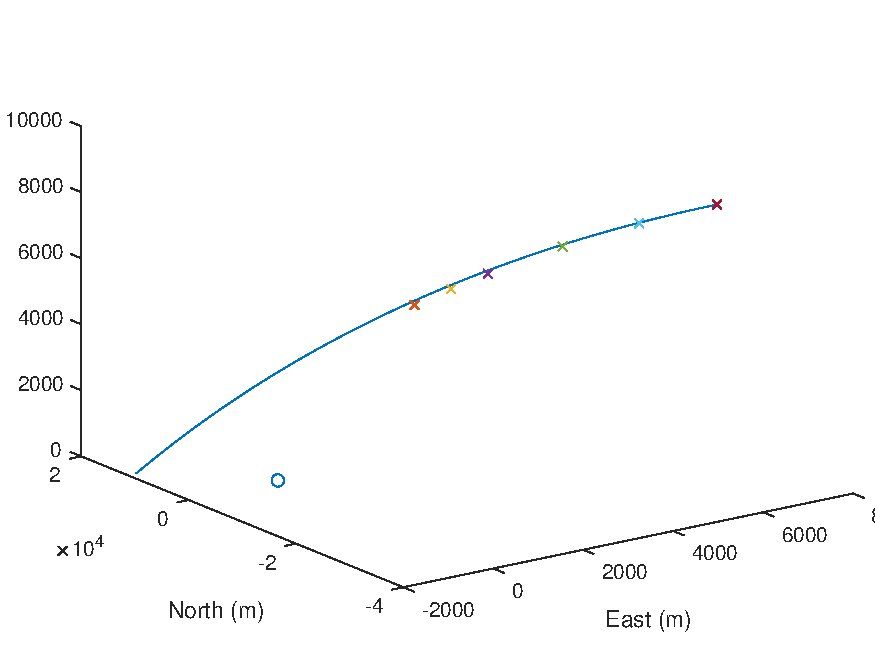
\includegraphics[width=\linewidth]{Figures/trajunpowatmo_1.pdf}
		\caption{Unpowered Initial Trajectory in Atmosphere \label{fig:trajunpowatmo_1} }
	\end{minipage}
\end{figure}

\begin{figure}[H]
	\centering
	\begin{minipage}{4.5 in}
		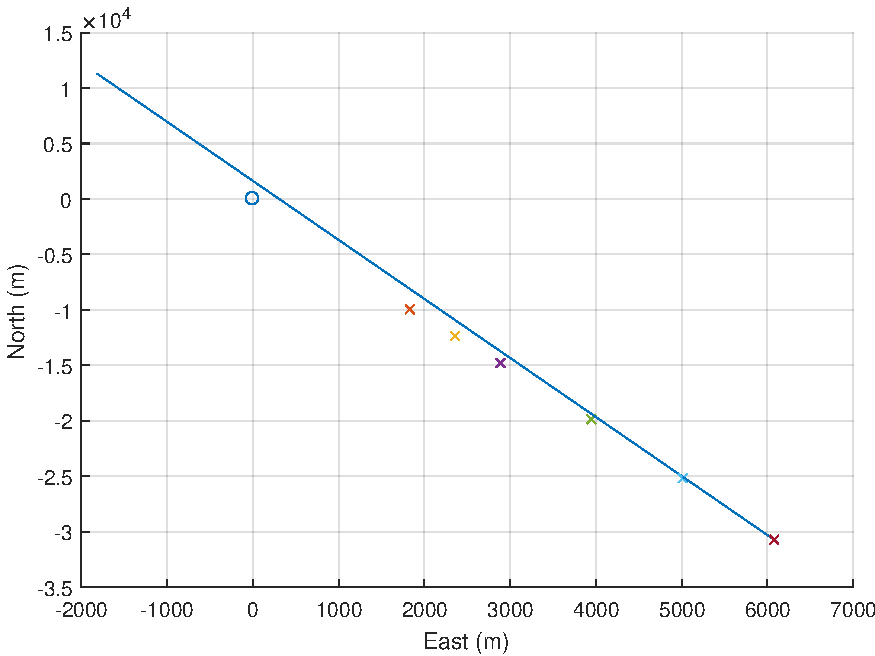
\includegraphics[width=\linewidth]{Figures/trajunpowatmo_2.pdf}
		\caption{Unpowered Initial Trajectory in Atmosphere From Above \label{fig:trajunpowatmo_2} }
	\end{minipage}
\end{figure}


%\section{Figures or How to Get into Real Trouble if You Take Advantage
%  of What \LaTeX\ Can Do}
%
%This section shows how to display figures and refer to them in the
%text.  \LaTeX\ does have the ability to insert postscript files using
%the \verb+graphicx+ package.  Make sure to include
%\verb+\usepackage{graphicx}+ in your preamble, that is between the
%\LaTeX\ commands \verb+\documentclass+ and
%\verb+\begin{document}+. \emph{See}
%  \verb+http://en.wikibooks.org/wiki/LaTeX/Importing_Graphics+
%  \emph{for information about importing graphics into your
%    document.}
%
%To insert a figure that is formatted in encapsulated postscript, which
%must include a Bounding Box line which is named \texttt{fname.ps} you
%do the following:
%\\
%\texttt{ \hspace*{0.5in} $\backslash$begin\{figure\}[ht]
%  \\
%  \hspace*{0.75in}
%  $\backslash$includegraphics[width=$\backslash$linewidth]\{fname.eps\}
%  \\
%  \hspace*{0.75in} $\backslash$caption\{Insert a caption
%  here. $\backslash$label\{figlabel\} \}
%  \\
%  \hspace*{0.5in} $\backslash$end\{figure\} }
%\\
%to produce the figure. The \textbf{[ht]} argument to the figure
%command is a \emph{suggestion} to \LaTeX\ to put the figure
%\textbf{[h]}ere, or at the \textbf{[t]}op of the page; \textbf{[p]}
%for a separate page is also possible.
%Avoid\marginpar{\small\textbf{\textit{Style note}}} putting tables and
%figures at the \textbf{[b]}ottom of the page as this is frowned upon
%by the thesis manual; the
%preference\marginpar{\scriptsize\raggedright\textbf{NEVER put anything
%    in the margin like this!!!}} is to put tables and figures right
%after they are first referenced, \emph{i.e.}\ \textbf{[h]}ere, but
%at the \textbf{[t]}op of the following page is acceptable in cases
%where it does not fit \textbf{[h]}ere.  You can make the suggestion
%stronger by saying \textbf{[h!]}  for ``\textbf{[h]}ere\textbf{!},''
%but the internal rules may still override your suggestion.
%``\verb+\linewidth+'' above can be replaced by some
%number of inches (or other size \LaTeX{} size measure such as
%\texttt{pt}, \texttt{em}, or \texttt{ex}).  This will left justify the
%figure.  Centering is a little more complicated.  We place everything
%in a \texttt{minipage} environment:
%\\
%\texttt{ \hspace*{0.5in} $\backslash$begin\{figure\}[ht]
%  \\
%  \hspace*{0.75in} $\backslash$centering
%  \\
%  \hspace*{0.75in} $\backslash$begin\{minipage\}\{$x$in\}
%  \\
%  \hspace*{1.0in}
%  $\backslash$includegraphics[width=$\backslash$linewidth]\{fname.ps\}
%  \\
%  \hspace*{1.0in} $\backslash$caption\{Insert a caption
%  here. $\backslash$label\{figlabel\} \}
%  \\
%  \hspace*{0.75in} $\backslash$end\{minipage\}
%  \\
%  \hspace*{0.5in} $\backslash$end\{figure\} }
%
%To demonstrate how the department would like to see figures in the
%thesis the following is provided. If you are examining these files
%with \texttt{xdvi}, you will only see a blank spot. However, both
%printed and ghostview methods described in the previous chapter will
%allow viewing.  Suppose that we create a figure to graph the curve
%\begin{equation}
%  y=\sin(\omega t), \label{gr1}
%\end{equation}
%where $\omega$ is the circular frequency.  Figure~\ref{fig1} is a
%graph of Equation~(\ref{gr1}), and figure~\ref{fig:graph} is an
%illustration of a mapping in the complex plane. The interval of time
%viewed is $t \in [-5,5]$. The figure reference should be denoted by
%either Fig.~\ref{fig1} or by Figure~\ref{fig1} with specific figures
%capitalized as noted here.
%%\begin{figure}[ht]
%%  \centering
%%  \begin{minipage}{4.5in}
%%    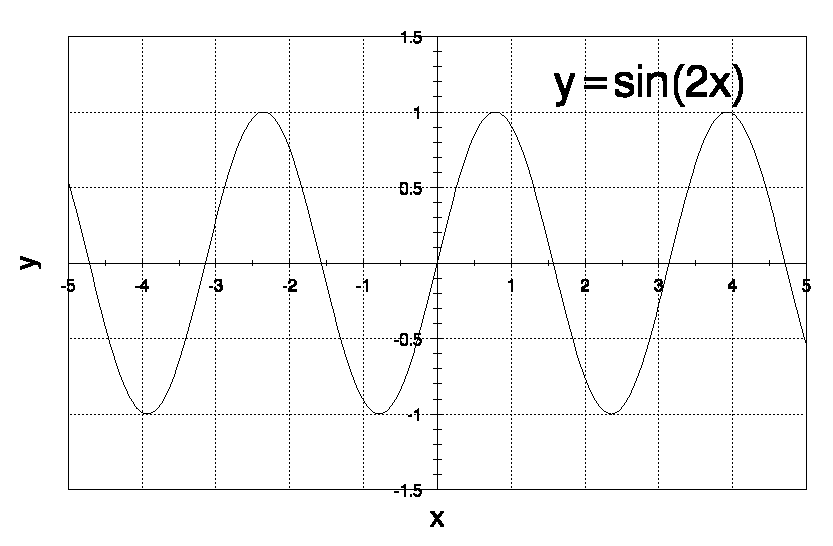
\includegraphics[width=\linewidth]{Figures/plot2.eps}
%%    \caption{This is a graph of the above equation, where the circular
%%      frequency is taken as $\omega = 2$.\label{fig1} Note: \emph{if
%%        you need to cite a source (of e.g.~a figure) in the caption,
%%        include the FULL CITATION, e.g.~} Source: Montezuma
%%      Publishing, San Diego State University Dissertation and Thesis
%%      Manual: Policies, Procedures and Format, Spring
%%      2010.\:\cite[\S 4.10.4 Figures]{DTM2010spring}}
%%  \end{minipage}
%%\end{figure}
%
%%\begin{figure}[ht]
%%  \centering
%%  \begin{minipage}{4.5in}
%%    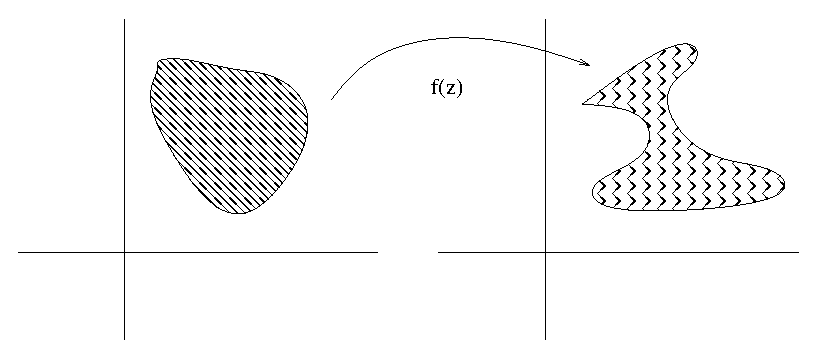
\includegraphics[width=\linewidth]{Figures/mapping.eps}
%%    \caption{Mapping $f(x)$ from the complex plane to itself. \label{fig:graph}}
%%  \end{minipage}
%%\end{figure}
%
%
%When you have a collection of figures and large figures, you may want
%to delay insertion of them until the end of the chapter. At the end of
%this chapter we are including a full page figure (Fig.~\ref{fullfig})
%to demonstrate this \LaTeX\ command. Note that if you cannot obtain
%postscript figures or are having too much trouble using the technique
%described above, then you can use the \verb+\vspace+ command to
%provide an empty space in the manuscript, then use the old-fashioned
%technique of taping in your figure and photocopying it.
%
%% 
%% If you have oversize full page figures, the following
%% might come in handy
%% 
%% \figurecoversheet{\label{figure:oversize} Caption goes here}
%
%
%\section{Tables}
%
%The Department of Mathematical Sciences does not have specific
%requirements on the exact layout of a table. However, the tables
%should be easily readable and properly labeled according to the
%regulations in the SDSU Thesis Manual. In this section we want to
%demonstrate how \LaTeX\ handles tables. More complicated examples can
%be found in Lamport's book\:\cite{LAM,LAM2}. We begin with a small table,
%given by Table\:\ref{tab1} which inserts nicely into the text.  Note
%that the same centering trick as was employed for figures is done here
%and we set the width of the \texttt{minipage} environment to 1.9
%inches.
%% 
%
%\begin{table}[hbt]
%  \centering
%  \begin{minipage}{1.9in}
%    \caption{A Small Table for Listing Some Parameters Used in Some
%      Numerical Procedure\label{tab1}. LONG CAPTION--- The Department
%      of Mathematical Sciences does not have specific requirements on
%      the exact layout of a table. However, the tables should be
%      easily readable and properly labeled according to the
%      regulations in the SDSU Thesis Manual.}
%    \begin{tabular}{|c||c|c|c|c||}    \hline
%      Trial &	a  &  b & c & $\omega$ \\ \hline \hline
%      1 & 5 & 10  & 15 & $\pi$ \\ \hline
%      2 & 10 & 20  & 15 & $2\pi$ \\ \hline
%    \end{tabular}
%  \end{minipage}
%\end{table}
%% 
%
%The\marginpar{\small\textbf{\textit{Style note}}} manual however
%allows for the caption to be a little wider if the table is really
%small and so we can use a wider \texttt{minipage} and then center the
%table inside there.  See for example Table\:\ref{wtab} where we used
%width of 3.5 inches.
%% 
%\begin{table}[hbt]
%  \centering
%  \begin{minipage}{3.5in}
%    \centering
%    \caption{Another Small Table for Listing Some Parameters Used in a
%      Numerical Procedure\label{wtab}.}
%    \begin{tabular}{|c||c|c|c|c||}    \hline
%      Trial &	a  &  b & c & $\omega$ \\ \hline \hline
%      1 & 5 & 10  & 15 & $\pi$ \\ \hline
%      2 & 10 & 20  & 15 & $2\pi$ \\ \hline
%    \end{tabular}
%  \end{minipage}
%\end{table}
%
%Note that you can use the \texttt{center} environment instead of
%\texttt{$\backslash$centering} but that might add a little bit of
%unwanted whitespace.  With \texttt{$\backslash$centering} on the other
%hand, you might have to put braces around the text you wish to center
%and sometimes need to add a \texttt{$\backslash$par}.  If you use it
%inside a \texttt{minipage}, \texttt{table} or \texttt{figure}
%environment, you don't have to really worry about that.  Note however
%that without the use of \texttt{minipage} you cannot center the
%caption as it automatically left aligns itself to conform with the
%thesis manual.
%
%Tables can also be left aligned see for example Table\:\ref{ltab}.
%Here we don't use the \texttt{minipage} environment, but we must then
%add linebreaks so that the table caption does not go wider then the
%table itself.  We need to add then two titles, one for the list of
%tables and one for the caption here.  The former will not have line
%breaks and the latter will.
%% 
%\begin{table}[hbt]
%  \caption[
%  Another Such Table but Left Aligned]{
%    Another Such\\Table but Left Aligned\label{ltab}}
%  \begin{tabular}{|c||c|c|c|c||}    \hline
%    Trial &	a  &  b & c & $\omega$ \\ \hline \hline
%    1 & 5 & 10  & 15 & $\pi$ \\ \hline
%    2 & 10 & 20  & 15 & $2\pi$ \\ \hline
%  \end{tabular}
%\end{table}
%
%Sometimes a table might not fit onto a single page, in this case you
%must not use the \texttt{table} environment, but instead the
%\texttt{longtable} environment.  Do note that \texttt{longtable}
%automatically centers so you need not worry about that.  See Table
%\ref{totallyrandom} for some absolutely random numbers.  To use
%\texttt{longtable} environment you must include the \texttt{longtable}
%package in your preamble. \textbf{see the note in \texttt{thesis.tex}
%  on how to fix the longtable entries in the ``List of Tables'' if
%  they are incorrect.}
%
%\begin{longtable}{|l|l|l|}
%  % You may need to modify the \LTcapwidth if the title wraps too early, or
%  % if it makes your table too large
%  % \LTcapwidth=6in
%  \caption{A Table of Some Totally Random Numbers} \label{totallyrandom} \\
%
%  % Here are our column headings
%  \hline
%  \multicolumn{1}{|l|}{\textbf{First}} &
%  \multicolumn{1}{l|}{\textbf{Second}} &
%  \multicolumn{1}{l|}{\textbf{Third}} \\
%  \hline \hline
%  \endfirsthead
%
%  % Here is the caption on other pages
%  \caption*{\tablename\ \thetable{} (Continued)} \\
%  \hline \multicolumn{1}{|l|}{\textbf{First}} &
%  \multicolumn{1}{l|}{\textbf{Second}} &
%  \multicolumn{1}{l|}{\textbf{Third}} \\ \hline \hline
%  \endhead
%
%  \multicolumn{3}{r}{\textbf{(table continues)}}
%  \endfoot
%
%  \hline
%  \endlastfoot
%
%  $16883.20050 \times 64.19591$ & $23174^{2905}$ & $(5112,5468,27117)$ \\ \hline
%  $7216.3398 \times 12239.16770$ & $19961^{9127}$ & $(16136,21997,26051)$ \\ \hline
%  $15977.29588 \times 5732.19698$ & $14995^{26728}$ & $(28634,14278,17183)$ \\ \hline
%  $24699.2338 \times 8803.18474$ & $19221^{28853}$ & $(18539,6044,19259)$ \\ \hline
%  $21444.11156 \times 24727.15793$ & $18372^{28126}$ & $(28032,2375,15319)$ \\ \hline
%  $4391.18511 \times 4548.30442$ & $1720^{1369}$ & $(3406,21419,16364)$ \\ \hline
%  $30135.17285 \times 30643.14550$ & $9216^{213}$ & $(23353,27690,19435)$ \\ \hline
%  $19438.13461 \times 25479.5929$ & $2137^{3868}$ & $(30657,17930,22240)$ \\ \hline
%  $26015.13194 \times 24615.8566$ & $17585^{10358}$ & $(13114,15259,12079)$ \\ \hline
%  $14483.18666 \times 730.30848$ & $16033^{18015}$ & $(28723,30583,27231)$ \\ \hline
%  $28936.21168 \times 22153.15603$ & $7838^{2847}$ & $(8315,13767,4984)$ \\ \hline$12183.11656 \times 22915.1655$ & $4903^{3341}$ & $(26271,13469,20927)$ \\ \hline
%  $3861.26584 \times 3418.15940$ & $8299^{22084}$ & $(16670,6379,5349)$ \\ \hline
%  $1917.2334 \times 3164.29148$ & $31271^{24332}$ & $(18534,14106,32170)$ \\ \hline
%  $21381.22421 \times 13170.26365$ & $1836^{24826}$ & $(16512,3492,29730)$ \\ \hline
%  $19854.29763 \times 10431.8013$ & $856^{4247}$ & $(11431,16797,12547)$ \\ \hline$748.699 \times 18926.6097$ & $2617^{21261}$ & $(9262,31765,19764)$ \\ \hline
%  $826.17531 \times 1102.229$ & $6144^{23524}$ & $(13399,32510,25360)$ \\ \hline
%  $5457.16254 \times 28852.2419$ & $3340^{25847}$ & $(12851,11353,26704)$ \\ \hline
%  $17098.22785 \times 10733.29645$ & $23533^{11432}$ & $(15804,29630,14049)$ \\ \hline
%  $4297.6124 \times 13047.24061$ & $6951^{30578}$ & $(25163,7180,3955)$ \\ \hline
%  $15919.20579 \times 3697.8512$ & $26036^{19951}$ & $(4596,28456,23292)$ \\ \hline
%  $30444.8539 \times 1877.24380$ & $25637^{24662}$ & $(2345,22515,15427)$ \\ \hline
%  $13777.5551 \times 12290.27827$ & $9848^{18414}$ & $(8106,1141,25365)$ \\ \hline$5916.26304 \times 32545.9871$ & $9456^{20356}$ & $(13568,17968,13625)$ \\ \hline
%  $752.22564 \times 9313.24044$ & $20240^{17852}$ & $(25921,11852,10721)$ \\ \hline
%  $17816.14197 \times 468.475$ & $27975^{6019}$ & $(12765,23034,15867)$ \\ \hline
%  $31180.31140 \times 17008.23777$ & $4288^{10545}$ & $(23555,14160,20001)$ \\ \hline
%  $11143.27728 \times 5201.24768$ & $28480^{27765}$ & $(1313,19756,15238)$ \\ \hline
%  $19165.12910 \times 27090.29887$ & $30726^{8520}$ & $(30355,31201,3727)$ \\ \hline
%  $3607.11199 \times 26761.19474$ & $9611^{25133}$ & $(3715,620,29421)$ \\ \hline
%  $14260.24175 \times 10813.1493$ & $2551^{5774}$ & $(6694,27319,1486)$ \\ \hline
%  $1691.28633 \times 21243.16929$ & $15030^{1385}$ & $(11252,12149,32111)$ \\ \hline
%  $19772.9737 \times 30544.23499$ & $13344^{8975}$ & $(17492,50,18586)$ \\ \hline
%  $9857.3765 \times 19207.6510$ & $18025^{10614}$ & $(17324,19518,13165)$
%
%\end{longtable}
%
%
%
%
%A larger table, given by Table\:\ref{tab2} and reproduced from another
%document, then you may need to allow an entire page for the
%table. This is done by typing the command
%\verb+\begin{table}[p]+. This test example is included in the
%minipage environment to show how a footnote\footnote{We also need to
%  see how a regular footnote appears in the text, so one was inserted
%  here. Multiple lines are easily handled by \LaTeX.}  can be added to
%a table.  Several problems have been noted before on how \LaTeX\
%handles the location of the table in the text.
%\begin{table}[p]
%  \centering
%  \begin{minipage}{3.7in}
%    \caption{Computations for Products of the \emph{RRN} Genes at Different
%      Growth Rates\label{tab2}}
%    \begin{tabular}{|c||c|c|c|c|c||}	 \hline
%      $\tau$(min)  &  100  &	60 & 40 & 30 & 24 \\ \hline \hline
%      $C$ period & 67 & 50  & 45 & 43 & 42 \\ \hline
%      $D$ period & 30 & 27  & 25 & 24 & 23 \\ \hline
%      $V_0$ & 0.437 & 0.577 & 0.815 & 1.15 & 1.63 \\ \hline
%      $\bar c$\footnote{$\times 1000\ {\rm ribosomes}/\mu{\rm m}^3$.}
%      & 11.1 & 16.8 & 22.1 & 28.1 & 31.4 \\ \hline
%      $\bar c_{85}$\footnote{$\times 1000\ {\rm ribosomes}/\mu{\rm m}^3$,
%        representing the average concentration of the product of the
%        \emph{rrn} gene located at $85'$.} & 1.73 & 2.68 & 3.65 & 4.81
%      & 5.57 \\ \hline 
%      $\bar c_{57}$\footnote{$\times 1000\ {\rm ribosomes}/\mu{\rm m}^3$,
%        representing the average concentration of the product of the \emph{rrn} gene
%        located at $57'$.} & 1.36 & 1.98 & 2.43 & 2.87 & 2.96 \\ \hline
%      $\bar c_{85}({\scriptstyle\times 100})/\bar c$\footnote{Percentage of
%        $\bar c$ produced by the \emph{rrn} gene located at $85'$.} & 15.6 & 15.9 &
%      16.5 & 17.1 & 17.7 \\ \hline
%      $\bar c_{57}({\scriptstyle\times 100})/\bar c$\footnote{Percentage of
%        $\bar c$ produced by the \emph{rrn} gene located at $57'$.} & 12.3 & 11.8 &
%      11.0 & 10.2 & 9.44 \\ \hline
%      $\bar c_{85}/\bar c_{57}$ & 1.27 & 1.35 & 1.50 & 1.68 & 1.88 \\ \hline
%      $r$\footnote{Initiations/min/gene.} & 3.75 & 10.27
%      & 22.56 & 38.42 & 56.98 \\ \hline
%      $c_{max}$\footnote{$\times 1000\ {\rm ribosomes}/\mu{\rm m}^3$, representing
%        the maximum concentration during the cell cycle.} & 11.28 & 17.04
%      & 22.33 & 28.36 & 31.77 \\ \hline
%      $c_{max}/c_{min}$\footnote{Ratio of maximum to minimum concentration
%        during the cell cycle.} & 1.041 & 1.036 & 1.027 & 1.024 & 1.026 \\ \hline
%    \end{tabular}
%  \end{minipage}
%\end{table}
%
%%\begin{figure}[p]
%%  \centering
%%  \begin{minipage}{4.5in}
%%    \includegraphics[width=\linewidth]{Figures/somb.eps}
%%    \includegraphics[width=\linewidth]{Figures/cos.eps}
%%    \caption{The top graph is the function $z = \sin(r)/r$, while
%%      the bottom surface is the function $z = \cos(r)$. \label{fullfig}}
%%  \end{minipage}
%%\end{figure}
%
%
%
%\section{Potential Pitfalls}
%
%\subsection{Tables and Figures}
%
%There is a conflict between the \verb+\usepackage{subfig}+,
%\verb+\usepackage{caption}+ and the \verb+sdsu-thesis.cls+ class
%specification.  The long table captions show up correctly (bold and
%left aligned with table).  Use \verb+\usepackage{subfigure}+ instead
%and all captions, as well as the list of tables page show up ok.
%
%If you insist on \verb+\usepackage{subfig}+, make sure to
%\textbf{first} issue the command
%\verb+\usepackage[bf,labelsep=period,textfont=bf]{caption}+ where the
%first "\verb+bf+" makes the labels "Figure n" bold;
%\verb+labelsep=period+ says "use '.' instead of ':'; and
%\verb+textfont=bf+ makes the caption text bold.  This may solve your
%subfig problems.
%
%
%Table captions (``table titles''\:\cite{DTM2010spring}) go
%ABOVE\marginpar{\small\textbf{\textit{Style note}}} the table, must be
%in \emph{headline style} where ``all major words are capitalized,''
%and there is no period at the end of the caption; in figure captions
%only the first word is capitalized, and there is a period at the
%end. --- \textbf{THE STYLE DOES NOT CURRENTLY ENFORCE THIS, \emph{YOU}
%  HAVE TO DO IT MANUALLY.}
%
%Charts, graphs, diagrams, maps, photographs, and other graphic
%illustrations should all be labeled as \emph{Figures}\:\cite[\S4.6.9,
%and \S4.10.4]{DTM2010spring}.  Figure captions are capitalized
%sentence style in the text; therefore, the List of Figures entries
%should be in sentence style.
%
%All tables and figures must be referenced in text \emph{prior} to
%their appearance. Those references should be by number.
%
%
%
%\subsubsection{Centered Tables Figures}
%\label{sec::centered:tab:fig}
%
%It is not as simple as adding \verb+\centering+ into the figure or
%table environment as that will center the caption on the page rather
%then left align it with the left edge of the figure or table.  So the
%way to solve this is to figure out the width of the figure or table
%and add it in a minipage and center that.  For example if our table is
%2 inches wide when typeset, then we could do
%\begin{verbatim}
%\begin{table}[ht]
%  \centering
%  \begin{minipage}{2in}
%    \caption{Caption goes here}
%    ... here is your table ...
%  \end{minipage}
%\end{table}
%\end{verbatim}
%
%
%
%\subsection{Margins}
%
%It is believed that the \verb+sdsu-thesis.cls+ template complies with
%the SDSU thesis manual: 1.25 inch left, 1 inch top, bottom and right.
%But your \emph{printout} may not give the right measurement, if your
%printer/printer-driver scales the document.  You may have to turn off
%scaling and/or tweak the settings in the \verb+sdsu-thesis.cls+ file.
%
%Someone said: \emph{``Some laser printers don't do the margins correctly, for
%example my printer shifts the page a bit.  You can correct this with
%the} \verb+\hoffset+ \emph{and} \verb+\voffset+ \emph{lengths as:}\\
%\hspace*{2em}\verb+\hoffset -0.0625in+\\
%\hspace*{2em}\verb+\voffset  0.15625in+''
%
%
%\subsection{Bad Pagebreaks}
%
%Sometimes LaTeX does not do exactly what you want with respect to
%pagebreaks.  To solve this you can manually add a \verb+\pagebreak+
%command where it should break, or you could add
%\verb+\enlargethispage{12pt}+ to make a page slightly larger if
%needed; though I'm not sure how the thesis reviewer will look on such
%transgressions, so do that at own risk.
%
%Bad pagebreaks in the table of contents (or list of tables/figures):
%If you get a bad pagebreak in a table of contents you can force a
%pagebreak by: \verb+\addtocontents{toc}{\protect\pagebreak}+ you add
%this at the point in your document that corresponds to that place in
%the table of contents.  For list of tables and list of figures,
%replace `toc' in the line above with `lot' or `lof.'
%
%
%\subsection{Bad Linebreaks}
%
%Bad linebreaks in chapter, section (subsection, etc...), or
%table/figure caption titles: This classfile tries to make all titles
%conform to the requirements of the thesis manual, but it is possible
%that it gets things wrong and  to add linebreaks (the
%\verb+\\+ command) yourself.  However, the table of contents title
%should not have any linebreaks.  The way you do it is to add an
%optional argument to \verb+\chapter+, \verb+\section+,
%\verb+\caption+ as in:\\
%\hspace*{2em}\textbf{$\backslash$chapter[Title for Table of
%  Contents]\{Title With$\backslash$$\backslash$Linebreaks\}}\\
%Note that for \verb+\caption+'s in figures and tables you might have
%to do this whenever you have a small figure or table as the
%table/figure environment cannot make the caption only as long as the
%figure since it doesn't know how large the figure is until it typesets
%everything.  See example above and more examples in the long-example
%directory.  You can also solve the \verb+\caption+ issue with minipage
%in the same way we do centering, see
%section~\ref{sec::centered:tab:fig}.
%
%
%
%\subsection{Vertical Space}
%
%This classfile tries to make all the vertical space as required, but
%sometimes you may need to modify what it does, or you just need to
%insert some vertical space.  You use the \verb+\vspace+ and
%\verb+\vspace*+ commands (see \LaTeX\ manual).  You can use positive
%or negative length there and \verb+\vspace*+ makes sure the space appears
%even if there is a pagebreak in between.  For example to add 2 inches
%of space you can add \verb+\vspace{2in}+.
%
%
%\subsection[Non-Bold Math in the TOC: $x=2\pi/e$]{Bold Math in the Thesis:  $\mathbf{x=\pi}$}
%
%Math in section titles need to be \textbf{bold}, but cannot be bold in
%the Table of Contents.

\chapter{RESULTS} \label{chap:results}
In this chapter results are presented for several simulated conditions.

\begin{enumerate}
	\item Nominal vs. dispersed parameters
	\item Atmosphere vs. vacuum
	\item Static initial conditions vs. Adaptive PDI
\end{enumerate}

The first condition, the effect of dispersion, is of interest on the topic of robustness. A closed-loop guidance law implementation is intended to ensure satisfaction of the problem constraints in practical conditions with uncertainty of state and performance limitations. A guidance system without periodic state feedback, i.e. an open-loop implementation, would be expected to quickly lose accuracy and ultimately fail in real application. Due to the criticality of safety in the intended mission, it is vital to show that the Adaptive PDI strategy performs well in nominal as well as dispersed conditions and to give a sense for the uncertainty in its performance.

The second condition is of particular interest because, as is clear in Section\:\ref{sec:guidancelaw}, neither APDG nor the PDI strategy take into account atmospheric effects and, at least in the case of the Apollo missions, have not been flown in the context of atmospheric landing. It is important to verify that the strategy can satisfy mission goals and still perform well in atmosphere, and the comparison with vacuum conditions serves both as a control as well as a fuel requirement baseline. 

The third condition is the subject of this study. Whether Adaptive PDI can reliably provide propellant efficiency improvement while maintaining safety and practicality is the topic of interest.

For dispersed cases the starting conditions are as listed in Table\:\ref{tab:IC} with the addition of Case 7, which represents the active PDI strategy. This Case is flown from the initial condition specified by Case 6, the first point on the trajectory, but with the engine off until one of the PDI criteria defined in Equations\:(\ref{eqn:thrustcriterion}) and\:(\ref{eqn:rangecriterion}) is met.

\subsection{Adaptive PDI} \label{sec:PDIres}
The first result to investigate is the validity of the PDI criteria in Equations\:(\ref{eqn:thrustcriterion}) and\:(\ref{eqn:rangecriterion}). For these criteria to serve as ignition criteria, they must reliably trigger in time to land the vehicle softly.

Figure\:\ref{fig:gtcriteriavac} shows data from a vacuum case of APDG with PDI active during the unpowered phase, before PDI has been triggered. The required thrust acceleration magnitude $a_{GT}$for a gravity turn is shown monotonically increasing throughout the unpowered trajectory, and the required downrange travel $s_{GT}$ is monotonically decreasing. $a_{GT}$ and $s_{GT}$ reach their limits at almost the same time, but this would not be true of all trajectories.


\begin{figure}[H]
	\centering
	\begin{minipage}{4.5 in}
		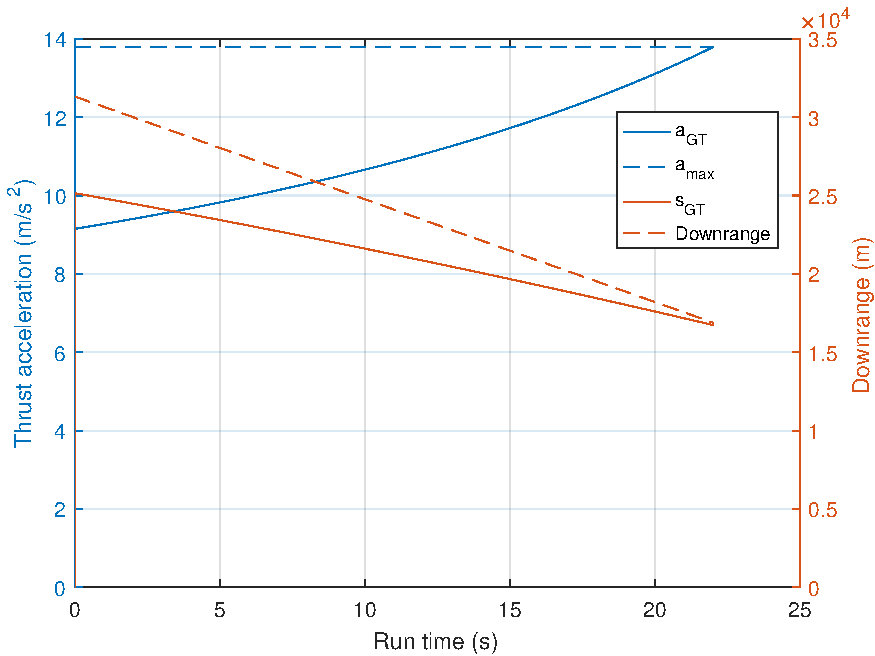
\includegraphics[width=\linewidth]{Figures/gtcriteriavac.pdf}
		\caption{PDI Criteria: Vacuum \label{fig:gtcriteriavac} }
	\end{minipage}
\end{figure}

Figure\:\ref{fig:gtcriteriaatmo} shows data from an atmospheric case of APDG with PDI active during the unpowered phase, before PDI has been triggered. Here the required thrust acceleration $a_{GT}$ is still monotonically increasing but not as quickly as it did in a vacuum, while $s_{GT}$ is decreasing similarly quickly. This behavior is examined in Section\:\ref{sec:atmovsvac}, where it is clear in Figures\:\ref{fig:altatmovsvac} and\:\ref{fig:spdatmovsvac} that the vehicle is able to provide significant lift while decelerating through drag during the unpowered phase in atmosphere. Figure\:\ref{fig:gtcriteriaatmo} clearly shows that the risk of overshoot, reflected in the downrange criterion, is much greater than exceeding the maximum thrust acceleration for this trajectory in atmosphere.

\begin{figure}[H]
	\centering
	\begin{minipage}{4.5 in}
		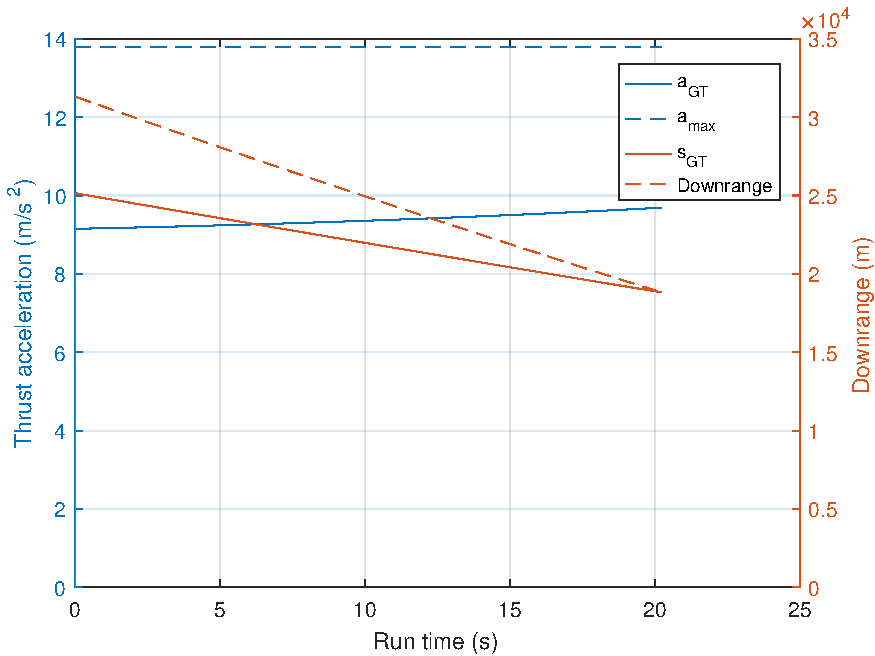
\includegraphics[width=\linewidth]{Figures/gtcriteriaatmo.pdf}
		\caption{PDI Criteria: Atmopshere \label{fig:gtcriteriaatmo} }
	\end{minipage}
\end{figure}


\subsection{Comparison of E-Guidance with APDG} \label{sec:lawcomp}
%Table and figures for the following condition:
%Both guidance laws
%Full dispersion (Rocket, IC, Nav)
%Atmospheric effects
%Dynamic Ignition Case
%Comparing guidance laws

The choice between E-Guidance of Equation\:(\ref{eqn:simplelaw}) as flown on the Apollo missions and APDG of Equation\:(\ref{eqn:APDGlaw}) is examined below. Results are first presented as nominal performance in atmosphere in order to investigate the individual performance of each law without the effects of dispersion. Beyond this section, results will be presented using APDG.

Figures\:\ref{fig:trajEvsAPDG} through\:\ref{fig:fatEvsAPDG} show plotted quantities of a rocket in atmosphere employing the PDI strategy on approach to landing at the origin from Initial Condition Case 6 (Table\:\ref{tab:IC}). In Figure\:\ref{fig:trajEvsAPDG} the trajectory with the steeper approach upon landing is flown by APDG. 

The laws each result in similar trajectories as evidenced by Figures\:\ref{fig:trajEvsAPDG} through\:\ref{fig:spdEvsAPDG}. However, the thrust profiles are notably different, with the APDG trajectory starting at a lower magnitude of thrust in Figure\:\ref{fig:thrEvsAPDG} than E-Guidance and their profiles roughly reversed. The pitch angle profiles in Figure\:\ref{fig:fatEvsAPDG} are very different with APDG providing a final pitch angle much closer to zero, indicating a level touchdown.

\begin{figure}[H]
	\centering
	\begin{minipage}{4.5 in}
		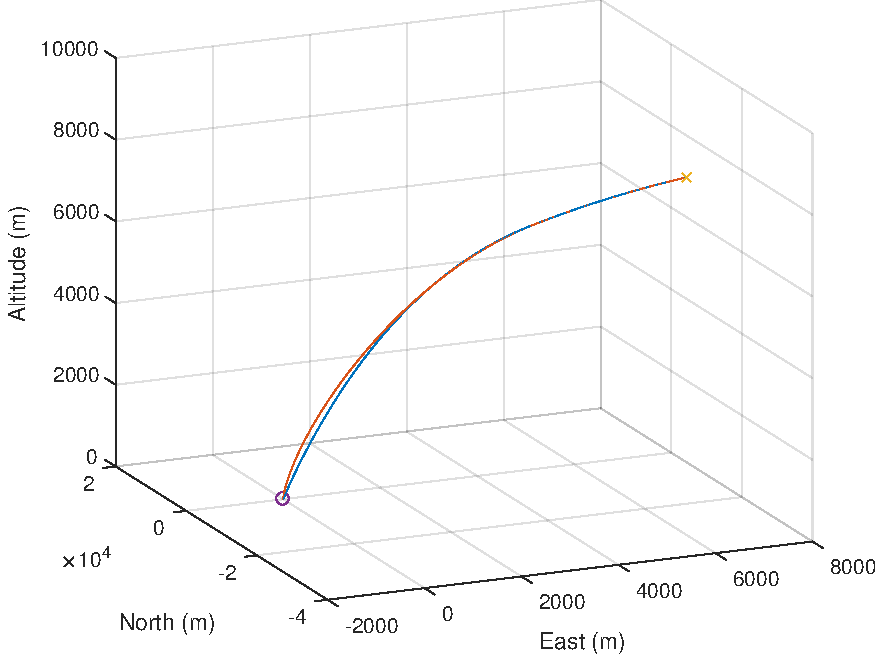
\includegraphics[width=\linewidth]{Figures/trajEvsAPDG.pdf}
		\caption{Trajectory: E-Guidance vs. APDG \label{fig:trajEvsAPDG} }
	\end{minipage}
\end{figure}

\begin{figure}[H]
	\centering
	\begin{minipage}{4.5 in}
		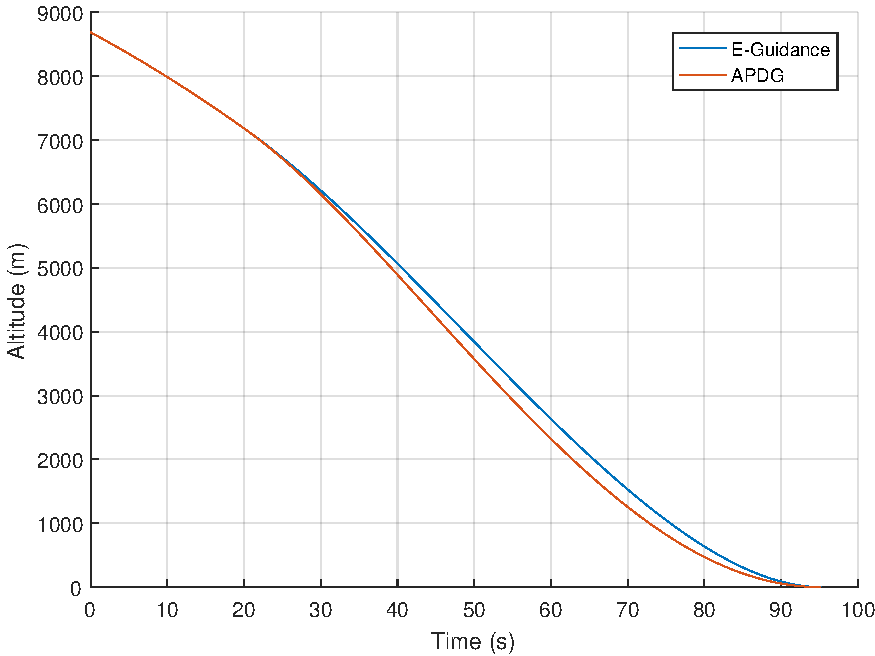
\includegraphics[width=\linewidth]{Figures/altEvsAPDG.pdf}
		\caption{Altitude: E-Guidance vs. APDG \label{fig:altEvsAPDG} }
	\end{minipage}
\end{figure}

\begin{figure}[H]
	\centering
	\begin{minipage}{4.5 in}
		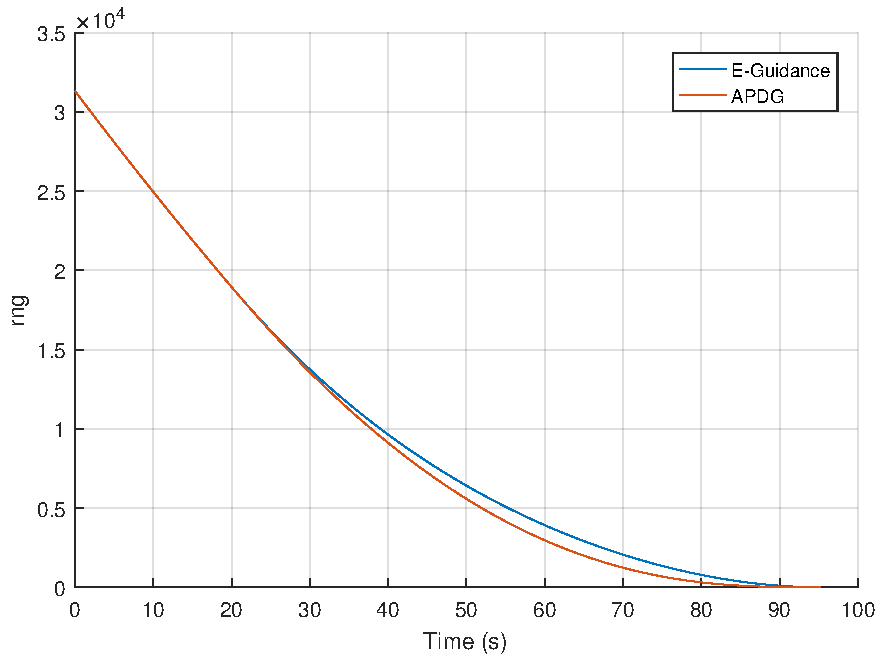
\includegraphics[width=\linewidth]{Figures/rngEvsAPDG.pdf}
		\caption{Ground Range: E-Guidance vs. APDG \label{fig:rngEvsAPDG} }
	\end{minipage}
\end{figure}

\begin{figure}[H]
	\centering
	\begin{minipage}{4.5 in}
		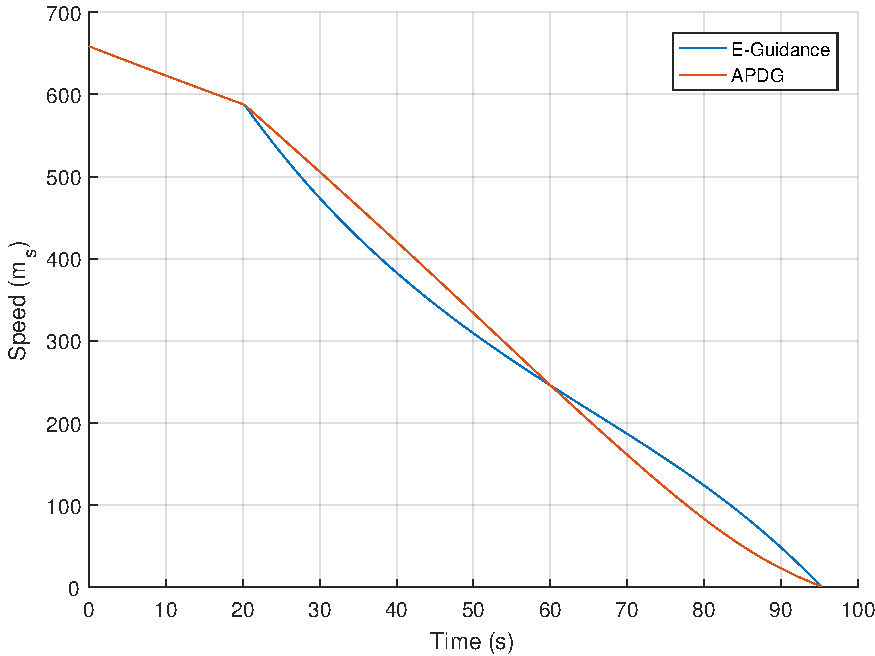
\includegraphics[width=\linewidth]{Figures/spdEvsAPDG.pdf}
		\caption{Speed: E-Guidance vs. APDG \label{fig:spdEvsAPDG} }
	\end{minipage}
\end{figure}

\begin{figure}[H]
	\centering
	\begin{minipage}{4.5 in}
		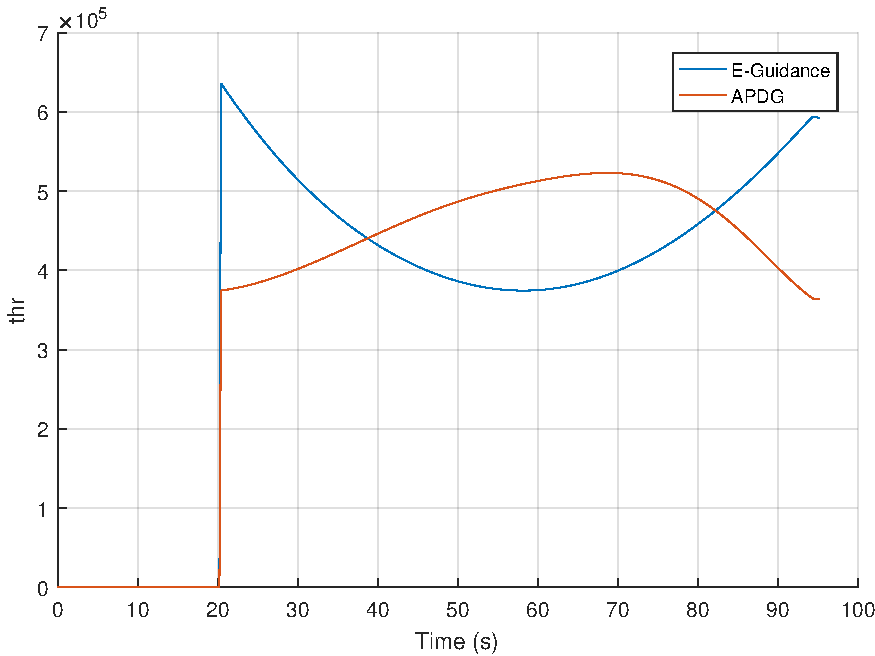
\includegraphics[width=\linewidth]{Figures/thrEvsAPDG.pdf}
		\caption{Thrust Magnitude: E-Guidance vs. APDG \label{fig:thrEvsAPDG} }
	\end{minipage}
\end{figure}

\begin{figure}[H]
	\centering
	\begin{minipage}{4.5 in}
		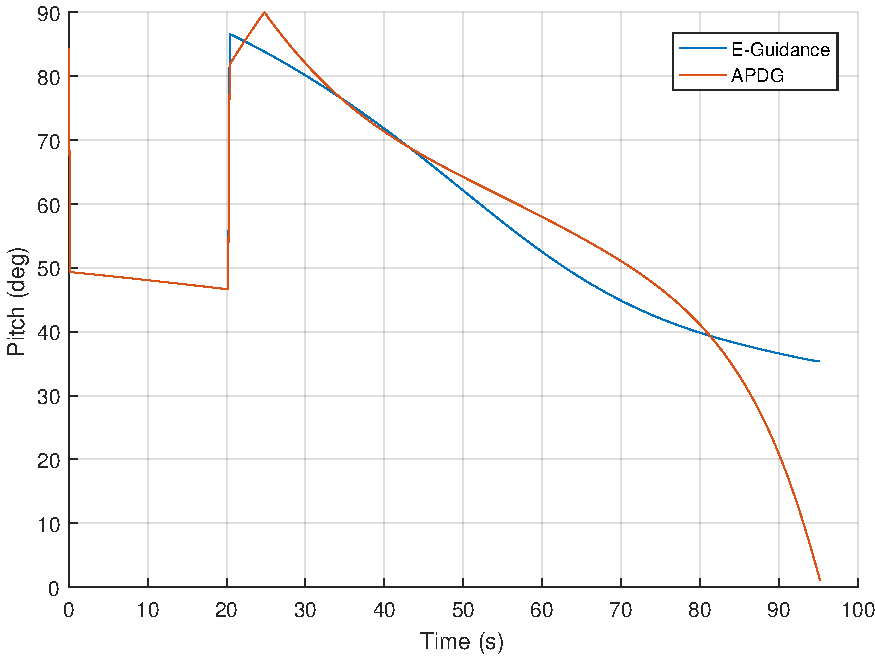
\includegraphics[width=\linewidth]{Figures/fatEvsAPDG.pdf}
		\caption{Pitch: E-Guidance vs. APDG \label{fig:fatEvsAPDG} }
	\end{minipage}
\end{figure}

Including dispersion results in similar profiles which will be examined more closely in later sections, but a numerical comparison of the laws' performance is given in Table\:\ref{tab:EvsAPDG}. Each law was in control for 1000 runs. Results are presented as mean values and standard deviations $\sigma$. Both laws perform similarly with the APDG law showing slightly higher speed on landing and using more fuel. This speed inaccuracy will be addressed in Section\:\ref{sec:naverror}

\begin{table}[ht]                                                                                              
	\centering        
	\caption{Comparison of Performance of E-Guidance with APDG}                     
	\label{tab:EvsAPDG}                                                                                              
	\begin{tabular}{|c|c|c|c|c|c|c|c|c|c|}                                                                         
		\hline                                                                                                        Guidance &      &   Fuel   &    Fuel   & Flight    &   FT     &  Range    &  Range   & Speed   &   Speed  \\ 
		Law      & Runs & (kg)      & $\sigma$ &  Time (s) & $\sigma$ &  (m) &    $  \sigma$ & (m/s)   & $\sigma$ \\
		
		\hline                                                                                                         
		E-Guidance  & 1000 & 9707.4 & 280.1 & 95.2 & 2.0 & 1.9 & 1.5 & 5.9 & 3.1 \\                                     
		\hline                                                                                                         
		APDG  & 1000 & 9849.8 & 287.3 & 95.0 & 2.0 & 2.5 & 1.9 & 8.0 & 3.6 \\                                       
		\hline                                                                                                         
	\end{tabular}                                                                                                  
	
\end{table}      

\subsection{Navigation Error} \label{sec:naverror}
%Table and figures for the following condition:
%APDG Guidance Law
%Rocket and IC Dispersion
%Atmospheric effects
%Dynamic Ignition Case
%Comparing Navigation Error vs. No Nav Error

The final speeds shown in Table\:\ref{tab:EvsAPDG} are not very accurate given the terminal velocity constraint magnitude of $1\:m/s$. This constraint is important since it determines how softly the vehicle will land. However, this final speed (and range) inaccuracy is due almost entirely to the navigation dispersion model outlined in Section\:\ref{sec:navmod}, as is clear from the results given in Table\:\ref{tab:navvsnonav}. Here the simulation was run with atmospheric effects, PDI, and full initial condition and rocket parameter dispersion. The cases differed only in whether navigation dispersion was active. The Nominal runs show very accurate satisfaction of the terminal constraints in spite of the guidance update stop for the last half second. A higher fidelity model would include much lower navigation error near the landing site due to the availability of more accurate measurements through radar systems and short range devices and would result in similarly low inaccuracies. More sophisticated sensor models are not investigated here since they would only apply near the end of flight, resulting in little impact on fuel consumption or performance of the PDI strategy.

\begin{table}[ht]                                                                                              
	\centering                             
	\caption{Comparison of Performance With and Without Navigation Error}                                          
	\label{tab:navvsnonav}                                                                          
	\begin{tabular}{|c|c|c|c|c|c|c|c|c|c|}                                                                         
		\hline                                                                                                        Nav &      &   Fuel    &    Fuel   & Flight    &   FT     &  Range    &  Range   & Speed   &   Speed  \\ 
		& Runs & (kg)      & $\sigma$  &  Time (s) & $\sigma$ &  (m) &    $  \sigma$ & (m/s)   & $\sigma$ \\
		
		\hline                                                                                                         
		Dispersed & 1000 & 9849.8 & 287.3 & 95.0 & 2.0 & 2.5 & 1.9 & 8.0 & 3.6 \\                                      
		\hline                                                                                                         
		Nominal & 1000 & 9761.8 & 270.8 & 95.2 & 2.0 & 0.1 & 0.0 & 1.0 & 0.0 \\                                   
		\hline                                                                                                         
	\end{tabular}                                                                                                  
	
\end{table}   

\subsection{Vacuum vs. Atmosphere} \label{sec:atmovsvac}
Here APDG's performance is compared with and without aerodynamic effects. This is an important comparison to make because, as stated in Section\:\ref{sec:EOMS}, the guidance law is derived without consideration of aerodynamic effects. There is no guarantee it will perform well in atmosphere. Only nominal results will be presented here, as the dispersed results are presented in Sections\:\ref{sec:vacperf} and\:\ref{sec:atmoperf} in the context of adaptive powered descent initiation (PDI) vs. predetermined ignition time.

Figures\:\ref{fig:trajatmovsvac} through\:\ref{fig:massatmovsvac} show nominal profiles for the APDG law in both atmosphere and vacuum. These trajectories start from Case 6 as listed in Table\:\ref{tab:IC}. Figures\:\ref{fig:trajatmovsvac} and\:\ref{fig:altatmovsvac} show that in atmosphere, the PDI strategy with the vehicle held at optimum angle of attack results in higher lift, meaning that the vehicle does not lose altitude as quickly as in vacuum, while Figure\:\ref{fig:spdatmovsvac} shows it losing speed much more quickly during this phase. This suggests that the aerodynamic effects have an appreciable effect on the energy in the form of propellant ultimately required for powered descent and soft landing. 

Figures\:\ref{fig:thratmovsvac} and\:\ref{fig:massatmovsvac} suggest the same conclusion. Upon ignition, the thrust required in atmosphere is far lower than that required in vacuum, and the ship mass stays higher in atmosphere throughout most of the trajectory, particularly the ending mass, reflecting lower fuel consumption. The thrust profile in atmosphere suggests a fairly conservative ignition; since more energy is burned off through aerodynamic effects, less thrust is required than might be expected by the gravity turn solution which generates the operative time-to-go. This leaves appreciable margin for error which is explored further in the dispersed results of Section\:\ref{sec:atmoperf}.


\begin{figure}[H]
	\centering
	\begin{minipage}{4.5 in}
		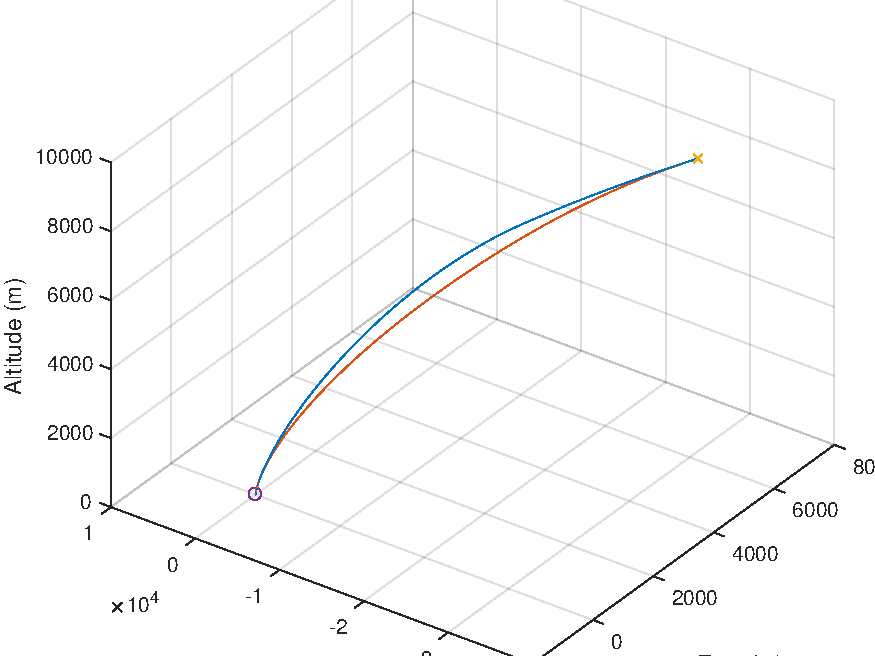
\includegraphics[width=\linewidth]{Figures/trajatmovsvac.pdf}
		\caption{Trajectory: Vacuum vs. Atmosphere \label{fig:trajatmovsvac} }
	\end{minipage}
\end{figure}

\begin{figure}[H]
	\centering
	\begin{minipage}{4.5 in}
		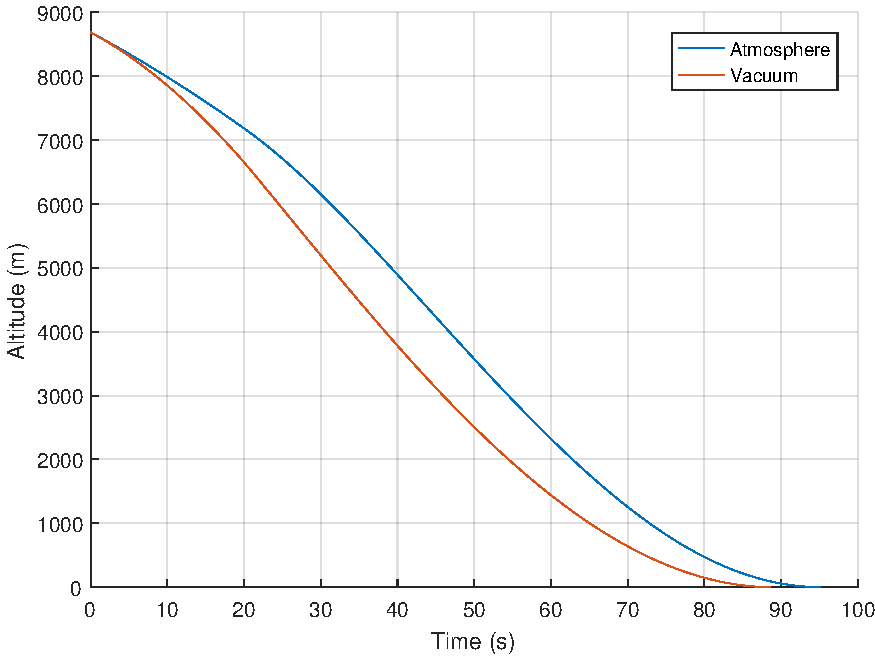
\includegraphics[width=\linewidth]{Figures/altatmovsvac.pdf}
		\caption{Altitude: Vacuum vs. Atmosphere \label{fig:altatmovsvac} }
	\end{minipage}
\end{figure}

\begin{figure}[H]
	\centering
	\begin{minipage}{4.5 in}
		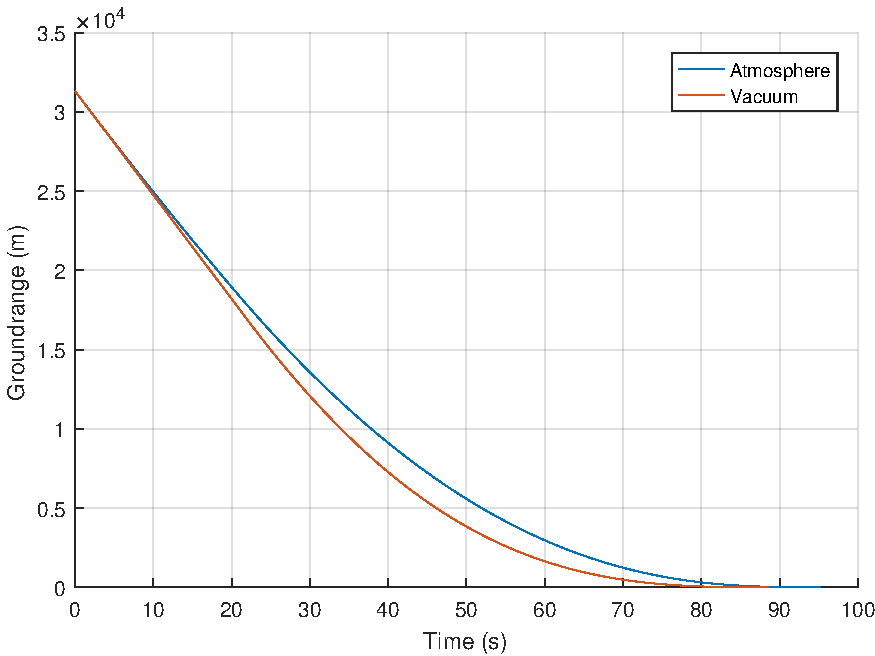
\includegraphics[width=\linewidth]{Figures/rngatmovsvac.pdf}
		\caption{Ground Range: Vacuum vs. Atmosphere \label{fig:rngatmovsvac} }
	\end{minipage}
\end{figure}

\begin{figure}[H]
	\centering
	\begin{minipage}{4.5 in}
		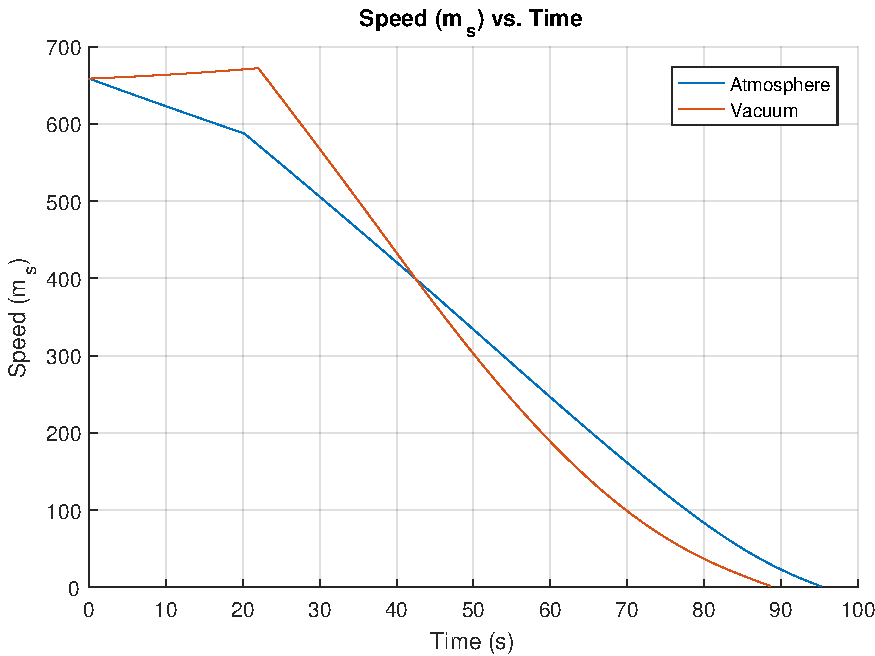
\includegraphics[width=\linewidth]{Figures/spdatmovsvac.pdf}
		\caption{Speed: Vacuum vs. Atmosphere \label{fig:spdatmovsvac} }
	\end{minipage}
\end{figure}

\begin{figure}[H]
	\centering
	\begin{minipage}{4.5 in}
		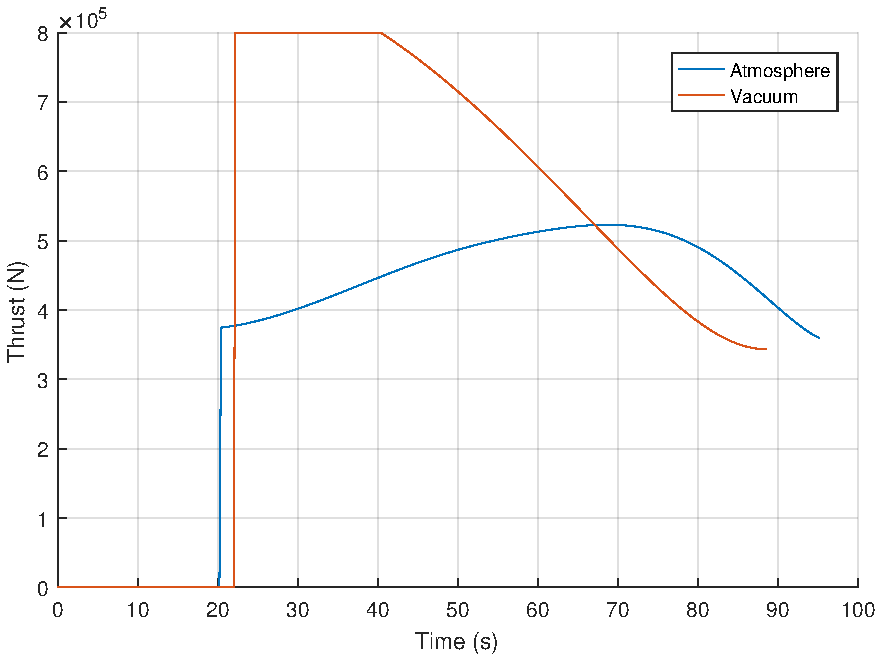
\includegraphics[width=\linewidth]{Figures/thratmovsvac.pdf}
		\caption{Thrust Magnitude: Vacuum vs. Atmosphere \label{fig:thratmovsvac} }
	\end{minipage}
\end{figure}

\begin{figure}[H]
	\centering
	\begin{minipage}{4.5 in}
		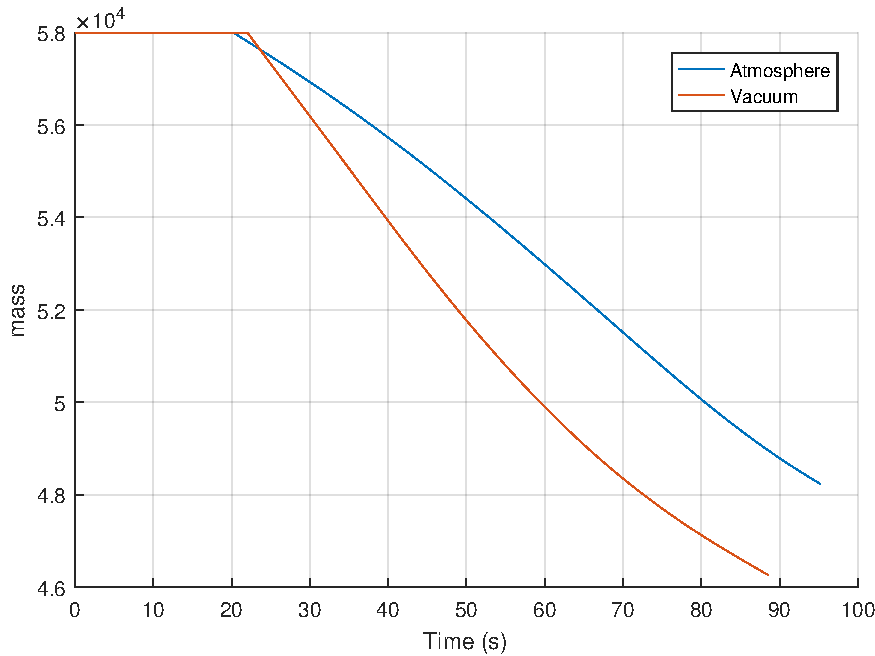
\includegraphics[width=\linewidth]{Figures/massatmovsvac.pdf}
		\caption{Ship Mass: Vacuum vs. Atmosphere \label{fig:massatmovsvac} }
	\end{minipage}
\end{figure}



\subsection{Vacuum Performance} \label{sec:vacperf}

%Table and figures for the following condition:
%APDG Guidance Law
%Full dispersion (rocket, nav, IC)
%Vacuum effects
%All cases including dynamic ignition
Presented here are results for the vacuum condition, comparing the performance and robustness of APDG with Adaptive PDI against specified ignition time in the form of predetermined initial conditions for a mission without aerodynamic effects. This is similar to the conditions experienced by the Apollo missions, though the simulation's parameters reflect a Martian gravitational field. As discussed in Section\:\ref{sec:guidancecomp}, there is a $1.2$ safety factor applied to the time-to-go as provided by Equation\:(\ref{eqn:tgoGT}) upon ignition for all cases in vacuum.

Figures\:\ref{fig:trajpowvac} through\:\ref{fig:thrpowvac} show nominal results for all cases. This gives a baseline from which to evaluate the typical profiles of each Case and the PDI strategy. 

Figure\:\ref{fig:trajpowvac} shows significant landing site overshoot on Case 1. The plot of Ground Range vs. Time in Figure\:\ref{fig:rngpowvac} tells a similar story, with the ground range nearly reaching zero before increasing at around 30 seconds before settling back toward zero. Figure\:\ref{fig:thrpowvac} is the most telling plot, with the Thrust Magnitude profiles for each case plotted vs. time. Cases 4 through 6 do not saturate at any point in their trajectories, either at the lower or upper bounds of thrust. Cases 1 through 3 do however, with Case 1 saturating at the upper bound for a large portion of its trajectory. 

Case 7 representing the PDI strategy also saturates its thrust for part of its trajectory after ignition but settles out toward the middle of the range by the end of its flight. Its other plots are unique relative to the other cases as well, with Speed in Figure\:\ref{fig:spdpowvac} showing the characteristic increase in speed due to its ballistic trajectory until powered descent initiation unlike all other Cases. Its Altitude in Figure\:\ref{fig:altpowvac} starts in line with Case 6 but decreases more quickly and ends on a similar path as Case 4. Its Ground Range behaves similarly in Figure\:\ref{fig:rngpowvac}. Its trajectory in Figure\:\ref{fig:trajpowvac} stands out in red, clearly following a much different path than any of the other Cases.

\begin{figure}[H]
	\centering
	\begin{minipage}{4.5 in}
		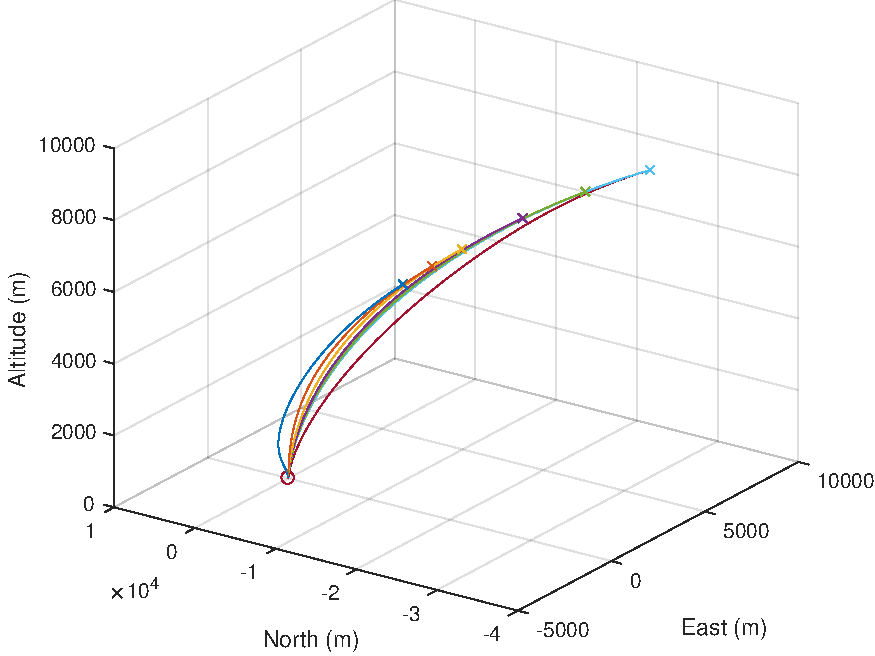
\includegraphics[width=\linewidth]{Figures/trajpowvac.pdf}
		\caption{Trajectory: APDG in Vacuum \label{fig:trajpowvac} }
	\end{minipage}
\end{figure}

\begin{figure}[H]
	\centering
	\begin{minipage}{4.5 in}
		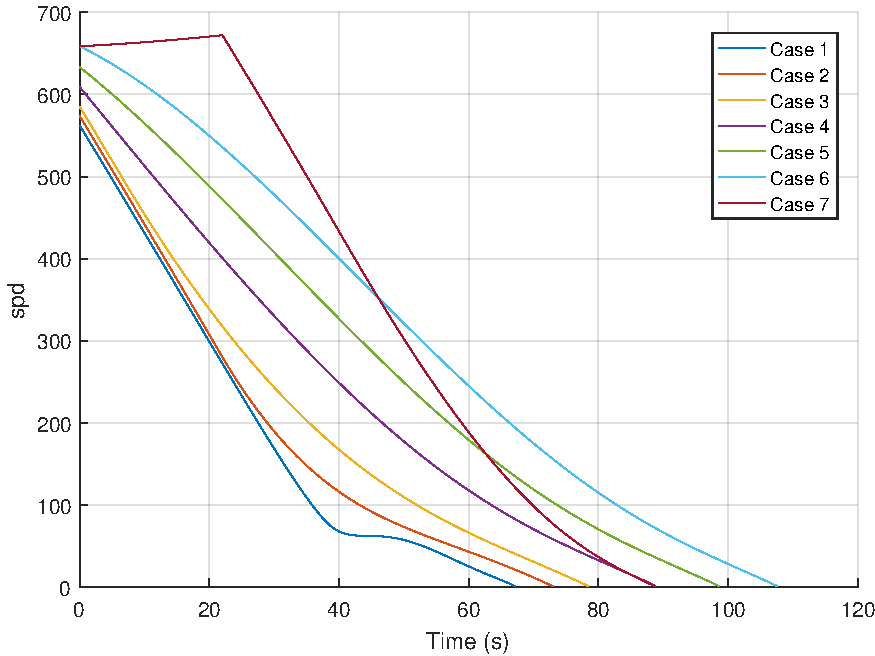
\includegraphics[width=\linewidth]{Figures/spdpowvac.pdf}
		\caption{Speed: APDG in Vacuum \label{fig:spdpowvac} }
	\end{minipage}
\end{figure}

\begin{figure}[H]
	\centering
	\begin{minipage}{4.5 in}
		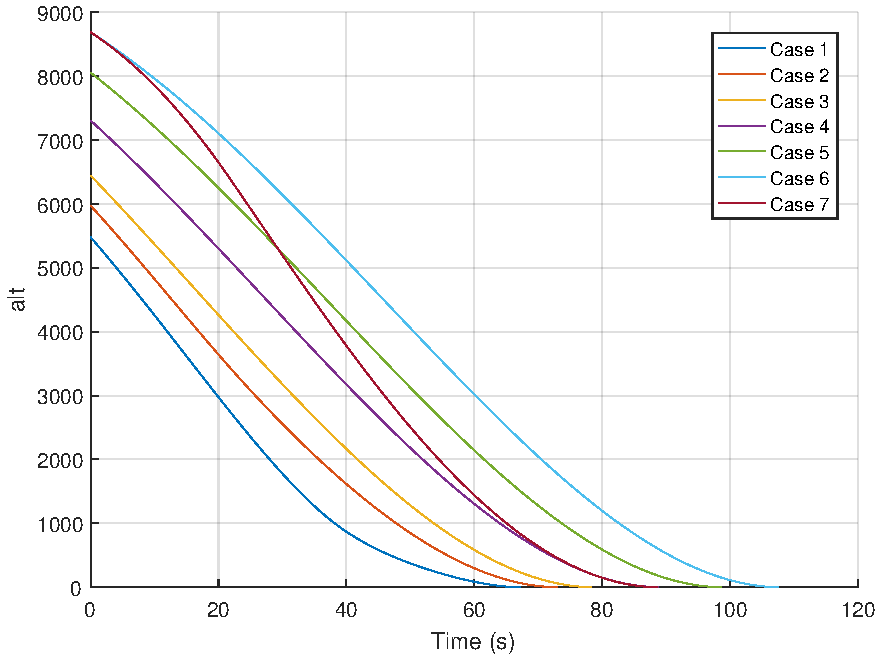
\includegraphics[width=\linewidth]{Figures/altpowvac.pdf}
		\caption{Altitude: APDG in Vacuum \label{fig:altpowvac} }
	\end{minipage}
\end{figure}

\begin{figure}[H]
	\centering
	\begin{minipage}{4.5 in}
		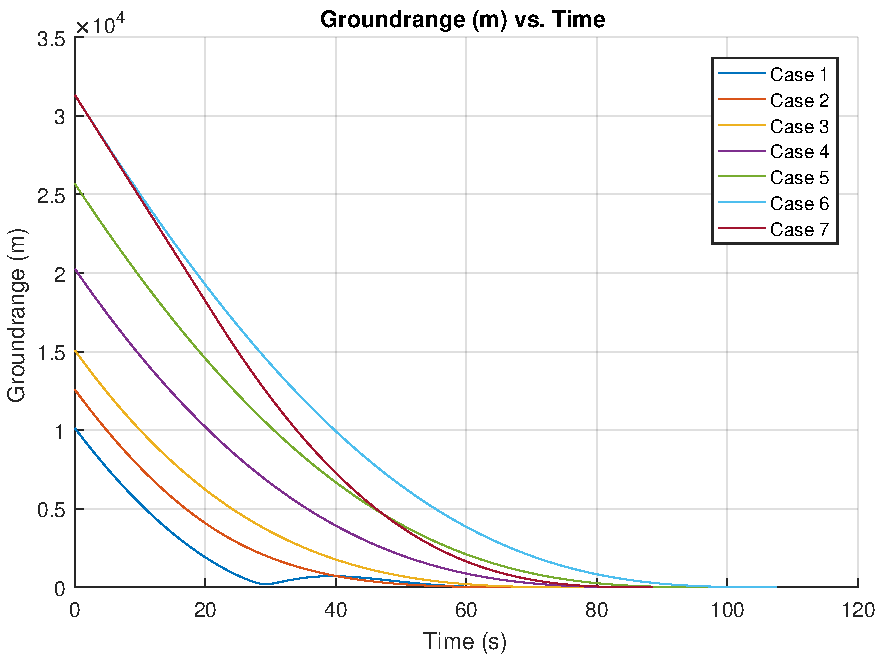
\includegraphics[width=\linewidth]{Figures/rngpowvac.pdf}
		\caption{Ground Range: APDG in Vacuum \label{fig:rngpowvac} }
	\end{minipage}
\end{figure}

\begin{figure}[H]
	\centering
	\begin{minipage}{4.5 in}
		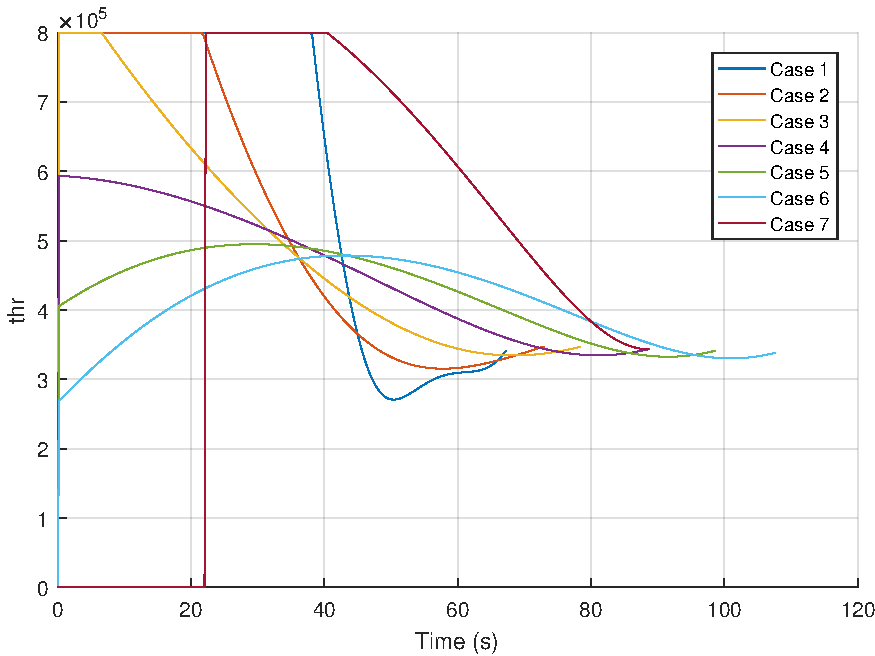
\includegraphics[width=\linewidth]{Figures/thrpowvac.pdf}
		\caption{Thrust Magnitude: APDG in Vacuum \label{fig:thrpowvac} }
	\end{minipage}
\end{figure}

Introducing dispersion gives the results in Table\:\ref{tab:disppowvac}. Most of the Cases perform similarly in terms of deviation from the mean aside from Case 1. Case 1 shows much higher fuel consumption deviation, flight time deviation, final range deviation, and final speed deviation. 

These deviations are due to failed landings; fully 45 of the 1000 runs of Case 1 in vacuum failed to land softly. All other runs had final ranges below 16 m, and all 45 of these failed landings had final ranges of over 600 m. Similarly, the 45 failed landings had final speeds in excess of 90 m/s, compared to the 16 m/s for all other Case 1 runs. Since the standard deviations of the other successful cases are in line with the errors expected from Navigation uncertainty in Section\:\ref{sec:naverror}, 16 m/s can be considered a bound on the error due to Navigation uncertainty, so these 45 landings are clearly cases where the guidance system failed.

None of the other cases had any such landing failures.

The lowest mean propellant consumption is given by Case 2, as well as the highest standard deviation in propellant consumption aside from Case 1.

\begin{table}[ht]                                                                                              
	\centering        
	\caption{Performance of PD Guidance In Vacuum}                                                                 
	\label{tab:disppowvac}                                                                                                                     
	\begin{tabular}{|c|c|c|c|c|c|c|c|c|c|}                                                                         
		\hline                                                                                                        Case &      &   Fuel   &    Fuel   & Flight    &   FT     &  Range    &  Range   & Speed   &   Speed  \\ 
		     & Runs & (kg)     & $\sigma$  &  Time (s) & $\sigma$ &  (m) &    $  \sigma$ & (m/s)   & $\sigma$ \\
		\hline                                                                                                         
		1 & 1000 & 11650.1 & 605.8 & 66.0 & 5.7 & 54.3 & 244.5 & 11.5 & 15.8 \\                                        
		\hline                                                                                                         
		2 & 1000 & 11184.7 & 308.2 & 72.7 & 3.4 & 2.5 & 2.0 & 8.3 & 3.7 \\                                             
		\hline                                                                                                         
		3 & 1000 & 11264.0 & 264.9 & 78.3 & 3.1 & 2.5 & 2.0 & 8.0 & 3.7 \\                                             
		\hline                                                                                                         
		4 & 1000 & 11634.4 & 247.0 & 88.9 & 3.1 & 2.6 & 2.0 & 8.3 & 3.8 \\                                             
		\hline                                                                                                         
		5 & 1000 & 12032.7 & 259.6 & 98.6 & 3.1 & 2.7 & 2.1 & 8.5 & 3.7 \\                                             
		\hline                                                                                                         
		6 & 1000 & 12436.7 & 241.9 & 107.7 & 3.0 & 2.5 & 2.1 & 8.3 & 3.8 \\                                            
		\hline                                                                                                         
		7 & 1000 & 11885.2 & 257.9 & 90.1 & 3.7 & 2.7 & 2.0 & 8.4 & 3.7 \\                                             
		\hline                                                                                                         
	\end{tabular}
\end{table}    

\subsection{Atmospheric Performance} \label{sec:atmoperf}
%Table and figures for the following condition:
%APDG Guidance Law
%Full dispersion (rocket, nav, IC)
%Atmospheric effects
%All cases including dynamic ignition

Presented here are results for the atmospheric condition, comparing the performance and robustness of APDG with Adaptive PDI against specified ignition time in the form of predetermined initial conditions for a mission with aerodynamic effects. This is representative of a Martian mission, the intended purpose of the CobraMRV. As discussed in Section\:\ref{sec:guidancecomp}, there is no safety factor applied to the time-to-go as provided by Equation\:(\ref{eqn:tgoGT}) upon ignition for any case in atmosphere. 

Figures\:\ref{fig:trajpowatmo} through\:\ref{fig:thrpowatmo} show nominal trajectories from each of the 6 Cases outlined in Table\:\ref{tab:IC} as well as Case 7 representing the Adaptive PDI strategy from the starting condition of Case 6. Figures\:\ref{fig:altpowatmo} and\:\ref{fig:spdpowatmo} show the behavior discussed in Section\:\ref{sec:atmovsvac} in which PDI's unpowered glide retains altitude while shedding speed. Figure\:\ref{fig:spdpowatmo} also shows odd behavior in Case 6, explained easily by Figure\:\ref{fig:thrpowatmo} in which the thrust saturates on the lower bound. Figure\:\ref{fig:thrpowatmo} shows PDI operating in the middle of the thrust range throughout the trajectory after ignition.

\begin{figure}[H]
	\centering
	\begin{minipage}{4.5 in}
		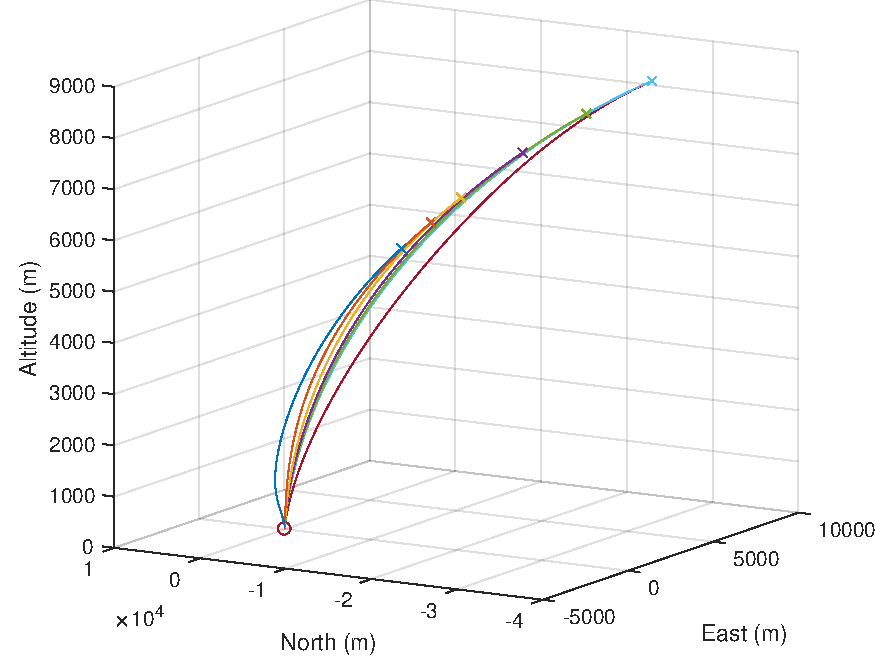
\includegraphics[width=\linewidth]{Figures/trajpowatmo.pdf}
		\caption{Trajectory: APDG in Atmosphere \label{fig:trajpowatmo} }
	\end{minipage}
\end{figure}

\begin{figure}[H]
	\centering
	\begin{minipage}{4.5 in}
		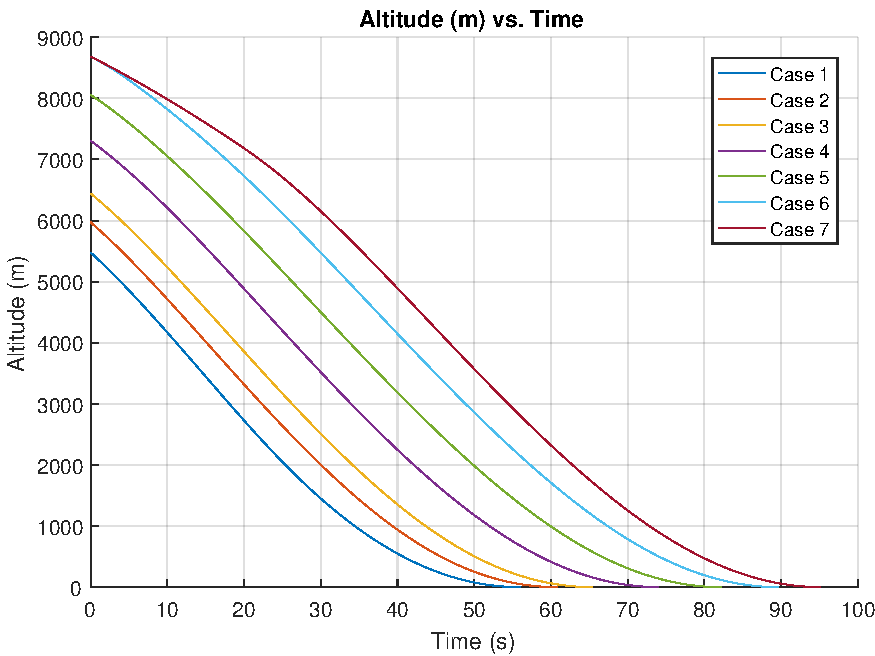
\includegraphics[width=\linewidth]{Figures/altpowatmo.pdf}
		\caption{Altitude: APDG in Atmosphere \label{fig:altpowatmo} }
	\end{minipage}
\end{figure}

\begin{figure}[H]
	\centering
	\begin{minipage}{4.5 in}
		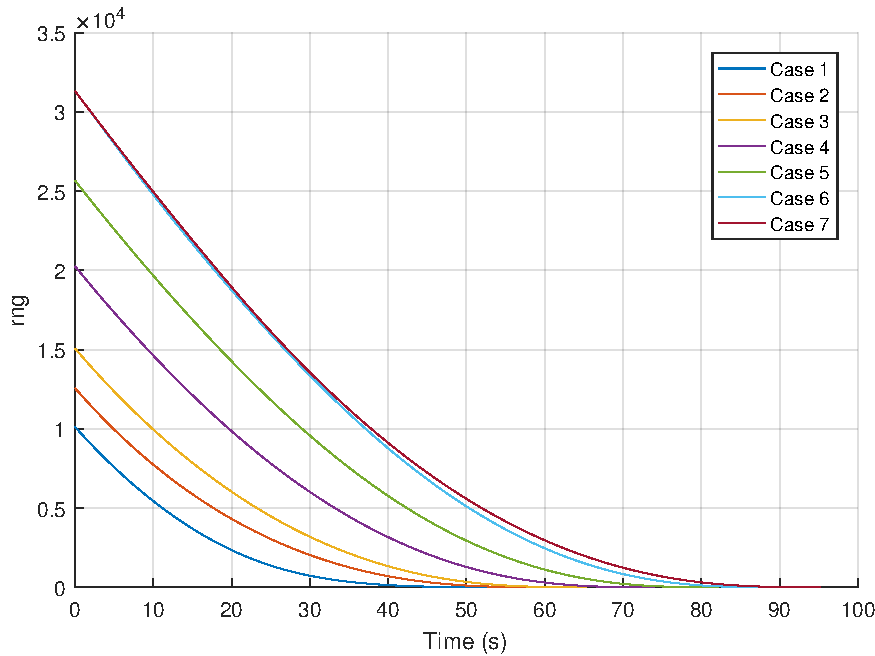
\includegraphics[width=\linewidth]{Figures/rngpowatmo.pdf}
		\caption{Ground Range: APDG in Atmosphere \label{fig:rngpowatmo} }
	\end{minipage}
\end{figure}

\begin{figure}[H]
	\centering
	\begin{minipage}{4.5 in}
		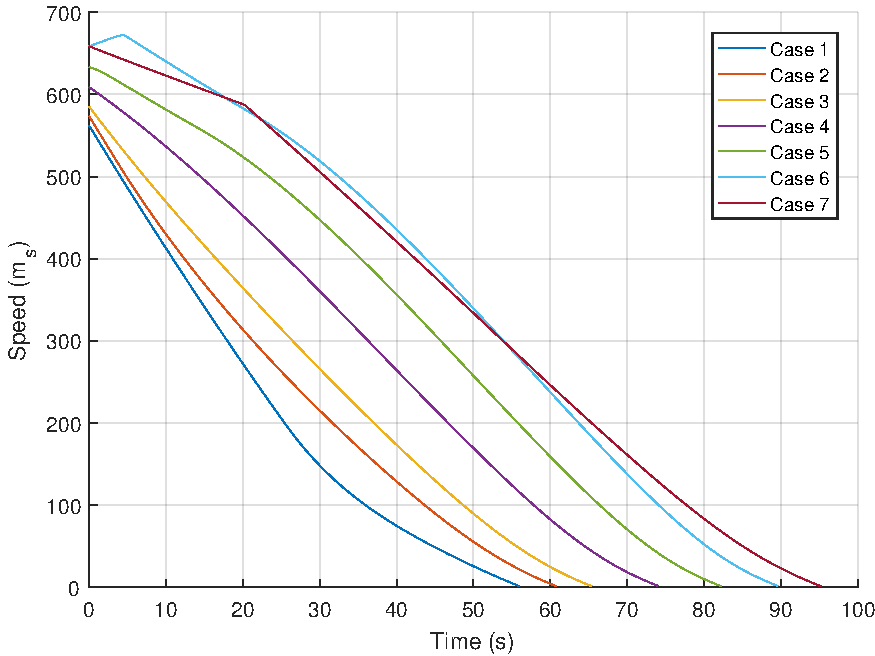
\includegraphics[width=\linewidth]{Figures/spdpowatmo.pdf}
		\caption{Speed: APDG in Atmosphere \label{fig:spdpowatmo} }
	\end{minipage}
\end{figure}

\begin{figure}[H]
	\centering
	\begin{minipage}{4.5 in}
		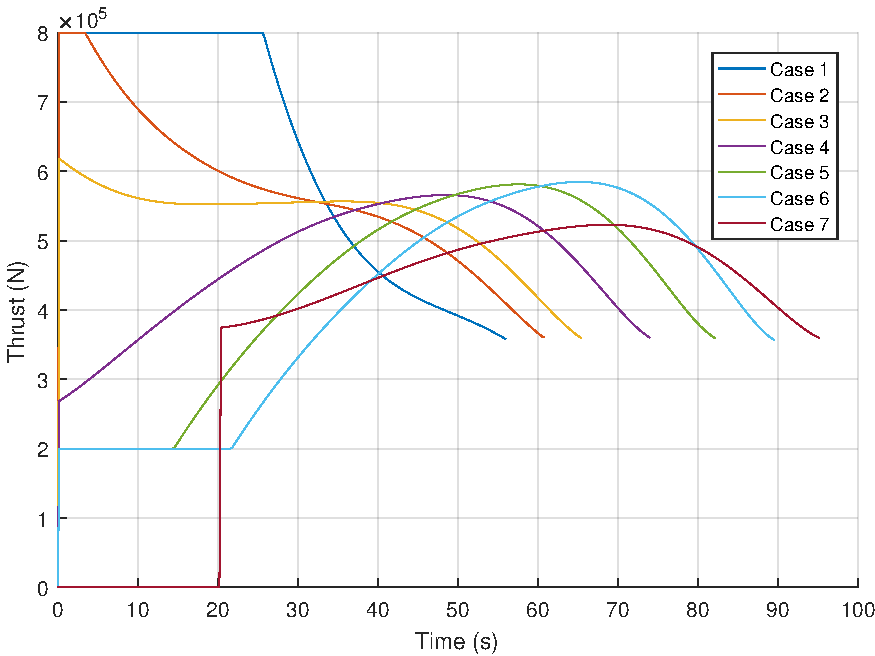
\includegraphics[width=\linewidth]{Figures/thrpowatmo.pdf}
		\caption{Thrust Magnitude: APDG in Atmosphere \label{fig:thrpowatmo} }
	\end{minipage}
\end{figure}

Introducing dispersion produces Table\:\ref{tab:disppowatmo}. Again we see Case 1 showing failed landings. In atmosphere only 13 landings of 1000 failed, with range misses in excess of 152 m and speeds in excess of 32 m/s. These values are lower than in vacuum.

PDI shows the best propellant performance in atmosphere, and no landing failures. Its final range and speed accuracy is well in line with the other Cases and the error introduced by Navigation uncertainty discussed in Section\:\ref{sec:naverror}.

\begin{table}[ht]                                                                                                  
	\centering        
	\caption{Performance of PD Guidance With Aerodynamic Effects}                                                  
	\label{tab:disppowatmo}                                                                                                
	\begin{tabular}{|c|c|c|c|c|c|c|c|c|c|}                                                                         
		\hline                                                                                                        Case  &      &   Fuel    &    Fuel   & Flight    &   FT     &  Range    &  Range   & Speed   &   Speed  \\ 
		      & Runs & (kg)      & $\sigma$  &  Time (s) & $\sigma$ &  (m) &    $  \sigma$ & (m/s)   & $\sigma$ \\
		\hline                                                                                                        
		1 & 1000 & 10141.2 & 357.5 & 55.8 & 3.2 & 9.1 & 60.2 & 8.8 & 7.4 \\                                            
		\hline                                                                                                        
		2 & 1000 & 9947.4 & 267.2 & 60.7 & 2.6 & 2.5 & 1.9 & 8.0 & 3.6 \\                                              
		\hline                                                                                                        
		3 & 1000 & 9918.5 & 264.8 & 65.4 & 2.8 & 2.6 & 1.9 & 8.2 & 3.5 \\                                              
		\hline                                                                                                        
		4 & 1000 & 9900.6 & 244.9 & 74.0 & 2.5 & 2.6 & 2.0 & 8.1 & 3.5 \\                                              
		\hline                                                                                                        
		5 & 1000 & 10010.2 & 217.6 & 82.0 & 2.7 & 2.5 & 1.9 & 8.1 & 3.5 \\                                             
		\hline                                                                                                        
		6 & 1000 & 10413.7 & 210.5 & 89.5 & 2.6 & 2.5 & 1.9 & 8.1 & 3.5 \\                                             
		\hline                                                                                                        
		7 & 1000 & 9849.8 & 287.3 & 95.0 & 2.0 & 2.5 & 1.9 & 8.0 & 3.6 \\                                              
		\hline                                                                                                        
	\end{tabular}
\end{table}   

\chapter{DISCUSSION} \label{chap:discussion}
%Here we interpret results, discussing agreement and disagreement with expected performance as well as sources of error and mitigation methods.

The results in Chapter\:\ref{chap:results} have many implications on the guidance approach of APDG as well as the adaptive powered descent initiation strategy of Section\:\ref{sec:PDI}. They will be discussed here, as well as the validity of the results themselves.

\section{Simulation Error Analysis} \label{sec:convergence}
As discussed in Section\:\ref{sec:RK4}, the numerical integration technique employed is a Runge-Kutta $4^{th}$ order method. This method is particularly attractive in computationally expensive applications because the total accumulated error due to time integration reduces on the order $O(\Delta t^4)$ where $\Delta t$ is the time integration step size, while the computational expense increases on the order $O(\Delta t)$. This means that a larger step size can produce the same order of error as an equally computationally expensive simulation using a first order scheme, saving significant computational and engineering time resources. There is a limit to the error reduction in that any finite computation produces machine error in rounding and variable storage. This simulation was run on a system with a machine error $\epsilon \approx 2*10^{-16}$.

To trust the validity of a simulation's results, it must be shown that the simulation is running within the numerical integration scheme's asymptotic convergence. In essence, the error should demonstrate the expected order behavior. 


A $4^{th}$ order scheme should show this error behavior. However, Figure\:\ref{fig:convtestatmo} clearly shows a linear error behavior, with error reducing with order $O(\Delta t)$. Error of order $O(\Delta t)$ and $O(\Delta t ^4)$ is shown for reference. This figure was generated by testing a particular moment in the simulation near the end of the trajectory without dispersion, with atmospheric effects and powered descent guidance. The baseline against which the error is measured is the a simulation result at the finest resolution, i.e. the smallest time step, $\Delta t = 2^{-13} \approx 1.2*10^{-4}$. Running the same test with an explicit $1^{st}$ order Euler scheme produces a similar result. 
\begin{figure}[H]
	\centering
	\begin{minipage}{4.5 in}
		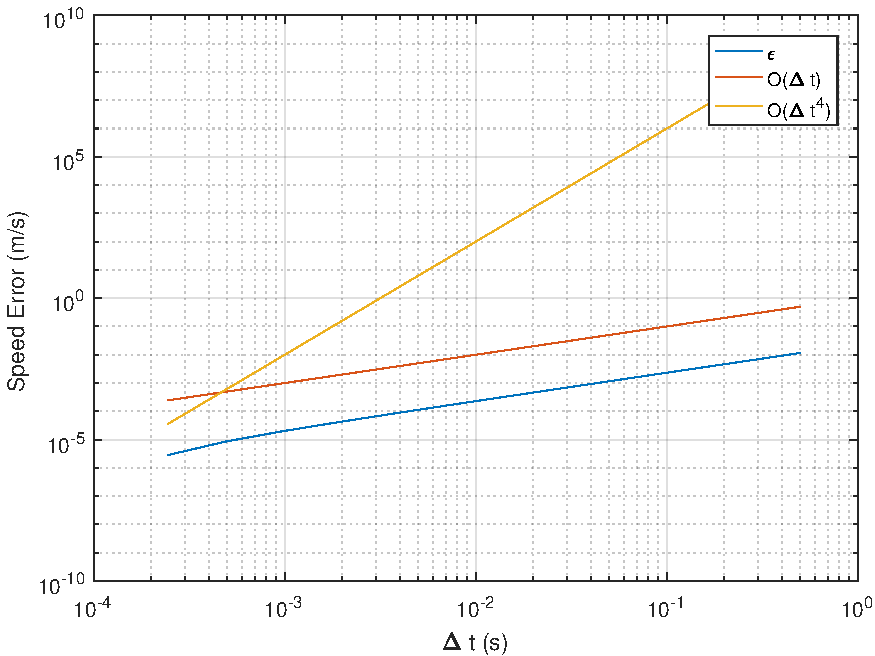
\includegraphics[width=\linewidth]{Figures/convtestatmo.pdf}
		\caption{Convergence Test: Powered in Atmosphere \label{fig:convtestatmo} }
	\end{minipage}
\end{figure}


The reason that the error does not show $O(\Delta t^4)$ behavior is that the derivative cannot be calculated at each intermediate step required for the RK4 scheme. Specifically, the terms $\bm{a}_T$ and $\frac{\bm{F}_{LD}}{m}$ representing the thrust acceleration and the aerodynamic effects in Equation\:(\ref{eqn:EoM_sim2}) must be held constant for the intermediate derivatives. These terms are actually also functions of the state $\bm{x}$, but they are highly non-linear. The thrust acceleration term is often actually held constant between steps since the guidance update rate is lower than the time integration rate, but every 200 time steps this assumption fails and error accumulates. Similarly, the aerodynamic model is never actually constant between time steps.

Holding terms which are functions of the state $\bm{\phi}$ constant between time steps reduces the integration method to Explicit Euler, given in Equation\:(\ref{eqn:euler}). 

\begin{equation}
\label{eqn:euler}
\bm{\phi}_{n+1} = \bm{\phi}_n + \Delta t \bm{f}(t_n,\bm{\phi}_n)
\end{equation}

If these terms are removed from the simulation, representing vacuum conditions with an unpowered trajectory, the error behavior is significantly different as demonstrated in Figure\:\ref{fig:convtestvac}. Here we see that the magnitude of the total error is drastically lower, a factor of $10^{-7}$ times the atmospheric error, yet no longer decreasing with $\Delta t$. This is because all remaining error in the solution is due to machine error for any practical time step size. Testing larger time steps would lead to unrealistic guidance update rates, making the simulation invalid or impractical.


\begin{figure}[H]
	\centering
	\begin{minipage}{4.5 in}
		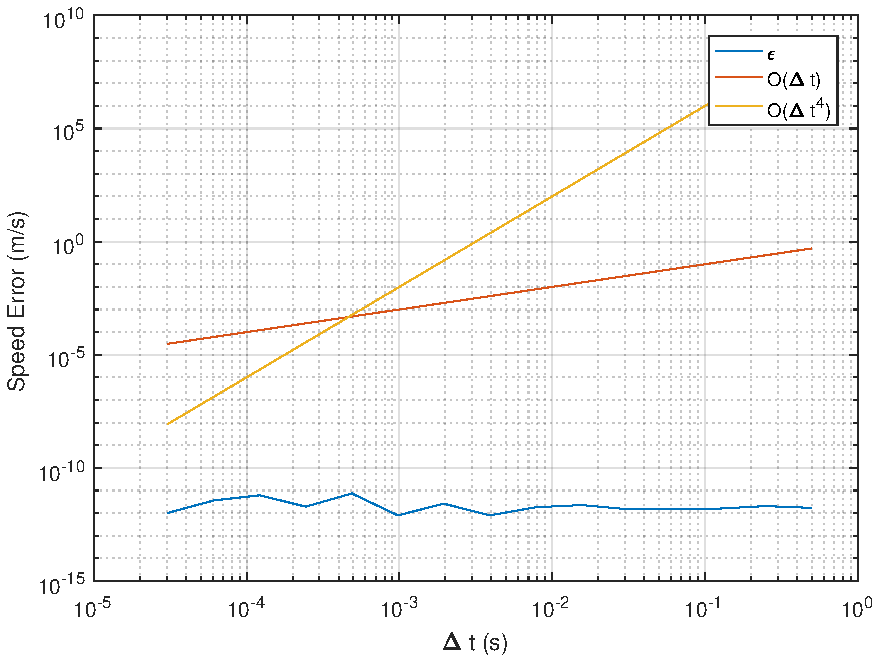
\includegraphics[width=\linewidth]{Figures/convtestvac.pdf}
		\caption{Convergence Test: Unpowered in Vacuum \label{fig:convtestvac} }
	\end{minipage}
\end{figure}

However, since the simulation error is dominated by the atmospheric and thrust acceleration terms and has reached the asymptotic convergence range for these terms, the results can be taken as valid.

\section{Apollo Powered Descent Guidance}
%The performance of APDG relative to E-Guidance is discussed here. The motivation is to show that, while not fuel optimal, it does produce reasonable results and can be expected to perform well while ensuring the practical mission consideration of final attitude constraints.

As shown in Section\:\ref{sec:optimality}, E-Guidance minimizes the performance index in Equation\:(\ref{eqn:performanceindex}). This index does not result in a fuel optimal guidance solution, but since it is penalizing large thrust accelerations it is doing something qualitatively similar. No claim is made about the optimality of the APDG solution, but it is clear in Table\:\ref{tab:EvsAPDG} that the propellant performance is comparable. Also clear is that the guidance solution is effective, meaning that the vehicle lands as softly and accurately under APDG as under E-Guidance. It may be slightly more sensitive to navigation error, but given quality navigation systems can be expected to satisfy terminal constraints very accurately, as shown in Table\:\ref{tab:navvsnonav}.

The primary motivation in choice of APDG is to ensure a practical final attitude. This aids in either landing the vehicle entirely under APDG or smoothly transitioning to a vertical descent guidance law. Figure\:\ref{fig:fatEvsAPDG} shows APDG's superiority to E-Guidance in this regard. APDG does a very good job of achieving nearly level vehicle orientation upon touch down. The pitch error still present is likely due almost entirely to the guidance command hold in place as described in Section\:\ref{sec:guidancecomp}, and would be easily dealt with. The significantly higher pitch error resulting from E-Guidance would have to be dealt with by another guidance phase specifically designed to ensure level landing, reducing the optimality of E-Guidance further.

\section{Adaptive Powered Descent Initiation} \label{sec:PDIdisc}
%The performance of PDI is examined. Discuss its raw propellant impact and explain the results (not the absolute lowest possible in vacuum, but the lowest in atmosphere). Discuss the failure of pre-determined ignition conditions in Case 1 and 6 and how PDI deals with this. Do this by examining both Case 1 as the "too late" condition and case 6 in atmosphere as the "too early" condition. Talk about how PDI can be adjusted to account for dispersions, atmospheres, etc. 

Section\:\ref{sec:PDIres} shows that the criteria in Equations\:(\ref{eqn:thrustcriterion}) and\:(\ref{eqn:rangecriterion}) are satisfied for the trajectories presented in Figure\:\ref{fig:trajunpowatmo_1}. It is clear that either the required thrust acceleration for a gravity turn $a_{GT}$ must at some point in the trajectory exceed the maximum thrust acceleration provided by the vehicle $a_{max}$, or the trajectory must be aligned such that the downrange distance to the landing site necessarily becomes smaller than the downrange distance traveled by a gravity turn maneuver $s_{GT}$. Figures\:\ref{fig:gtcriteriavac} and\:\ref{fig:gtcriteriaatmo} show that one or both of these requirements are satisfied. Further, it can be shown that one of these criteria will always trigger ignition for PDI. This is because $a_{GT}$ reflects, at minimum, the acceleration required to slow the vehicle from its current speed to the final landing speed. Since the PDI approach uses the time-to-go provided by a gravity turn maneuver, as the altitude approaches zero the time-to-go also approaches zero. With an increasing speed due to a ballistic trajectory and a decreasing time to go, $a_{GT}$ will obviously increase until it crosses the threshold $a_{max}$. Similarly, if the thrust acceleration criterion is not triggered, the trajectory will necessarily overshoot the landing site. Since the downrange distance traveled is roughly proportional to the speed squared as in Equation\:(\ref{eqn:rangeGT}), the range criterion will be triggered at some point before overshoot.

Confident that Adaptive PDI will trigger, the question of its performance arises. For vacuum, Table\:\ref{tab:disppowvac} shows PDI's propellant performance (Case 7) as middle-of-the-road compared to the other predetermined starting points. However, without knowledge of these results each starting point may seem as feasible as the others. Indeed, driving the initial condition closer to the landing site along the trajectory in Figure\:\ref{fig:trajunpowatmo_1} seems ideal as the propellant requirement drops according to Table\:\ref{tab:disppowvac}, with the minimum occurring for Case 2. But driving the ignition point too close to the landing site can result in unacceptable failure rates. Case 1 results in failures 45 out of 1000 runs, or a rate of $4.5\%$, wildly dangerous for a manned mission. Even in vacuum PDI provides decent fuel performance and removes the guesswork inherent in choosing predetermined ignition conditions.

In atmosphere PDI's advantage grows as evidenced by Table\:\ref{tab:disppowatmo}. Not only does Case 1 show an unacceptable manned mission failure rate of $1.3\%$, but PDI actually provides the best propellant performance of any Case. PDI's fuel savings come primarily from its unpowered flight. During the first 20 seconds in Figure\:\ref{fig:thrpowatmo} PDI does not burn any fuel, but it manages to reduce speed and altitude for free in Figures\:\ref{fig:spdpowatmo} and\:\ref{fig:altpowatmo}. Figure\:\ref{fig:massatmovsvac} comparing ship mass for the vacuum and atmospheric conditions using PDI shows the cumulative, increasing savings from aerodynamic effects.  In thicker atmospheres one should expect larger savings since PDI automatically takes advantage of these effects. Rather than risking failure for reduced propellant consumption, PDI ensures safety and performance.



%Middle chapter.  Here we put the middle things, that is, things that
%are in the middle and not in the beginning or in the end.  Here we
%also test all the section, subsection, and other headings.
%
%\textbf{Note\marginpar{\small\textbf{\textit{Style note}}} that
%  CHAPTER TITLES need to be in ALL CAPS --- YOU have enter the chapter
%  titles in ALL CAPS!!!}
%
%\section{A Section}
%
%Some section text.  Note that there should ALWAYS be some text in
%between two sectioning levels; a \verb+\section+ directly followed by
%a \verb+\subsection+ will not go through the review.
%
%\subsection{A Subsection With a Very Long Title To See How That Will
%  Look When Printed}
%
%Some subsection text.
%
%\subsubsection{A Subsubsection}
%
%Some subsubsection text.
%
%\subsubsubsection{A Subsubsubsection}
%
%Some subsubsubsection text.  If you are using this, you are
%\sout{probably} over-organizing things.
%
%\paragraph{A Paragraph.}
%
%Some paragraph text.  You never really get this deep --- don't be
%ridiculous.

\chapter{CONCLUSIONS AND FUTURE WORK} \label{chap:conclusions}
This chapter discusses the implications of the Adaptive PDI strategy and its wider applicability to guidance laws beyond APDG or E-Guidance. Section\:\ref{sec:futurework} recommends future study of PDI and particular avenues to explore.

\section{Adaptive Powered Descent Initiation}
As discussed in Section\:\ref{sec:PDIdisc}, PDI helps provides good fuel performance as well as a safety margin in combination with APDG. However, any guidance system operating with a vehicle subject to thrust acceleration limits as in Equation\:(\ref{eqn:thrustlimit}) would benefit from use of the Adaptive PDI strategy. Indeed, Lu recommends this PDI strategy in cooperation with his propellant optimal guidance solution\:\cite{LU}. For a lower bound limit, once the engine is ignited there is an absolute minimum amount of fuel that will be consumed. PDI helps reduce that minimum by not igniting the engine until necessary. For the upper bound limit, PDI ensures that the engine is ignited in time to land safely, while predetermined ignition Cases as in Table\:\ref{tab:IC} make no such assurances. These cases can be chosen carefully but there are inherently open-loop and cannot adjust to dispersed conditions resulting from trajectory errors or unexpected rocket parameter dispersions like reduced thrust performance in transit to the mission target planet.

PDI's closed-loop strategy which actively takes into account current vehicle conditions is invaluable for a manned mission to Mars, where there may be little opportunity to adjust mission phase plans on-line but where safety and fuel performance are of critical importance. 



\section{Future Work} \label{sec:futurework}
%Discuss refinements to PDI; tgo safety factor as function of conditions for mission planning, or directly optimal approach of some kind.

The wider applicability of PDI should be studied further. In particular, there are two major variables for implementation of PDI which depend upon proper mission planning. These variables reflect PDI's handling of the upper and lower thrust acceleration limits as well as the strength of aerodynamic effects.

The first is the time-to-go safety factor $c_t$ as described in Section\:\ref{sec:Time-to-go} which helps address the thust acceleration magnitude upper limit as demonstrated in Figure\:\ref{fig:thrtgofac} showing the thrust profiles of a vacuum trajectory with Adaptive PDI and APDG. With $c_t = 1.0$, the vehicle attempts a landing that requires too much thrust acceleration to achieve within the given time. This results in Figure\:\ref{fig:spdtgofac}, a plot of the speed profiles. With $c_t = 1.2$ the vehicle lands softly. This is because the time-to-go model assumes the only forces acting on the vehicle are thrust acceleration and gravitational acceleration, and plans for maximum thrust without landing site constraints, but the addition of trajectory error introduces unexpected work that needs to be done by the vehicle and the time-to-go is not large enough to allow it. Applying a safety factor accounts for the additional trajectory error and the vehicle lands softly. For the vacuum condition a factor $c_t = 1.2$ was necessary to provide a safety margin against the modeled dispersions including the landing site trajectory error, but in atmosphere it was not necessary and $c_t = 1.0$ was sufficient since some of the momentum dissipation is provided by aerodynamic effects. Ideally this factor would be automatically generated from mission conditions. For example, $c_t$ could be a function of atmospheric density or some other parameter to represent the work done throughout the trajectory by aerodynamic effects.

\begin{figure}[H]
	\centering
	\begin{minipage}{4.5 in}
		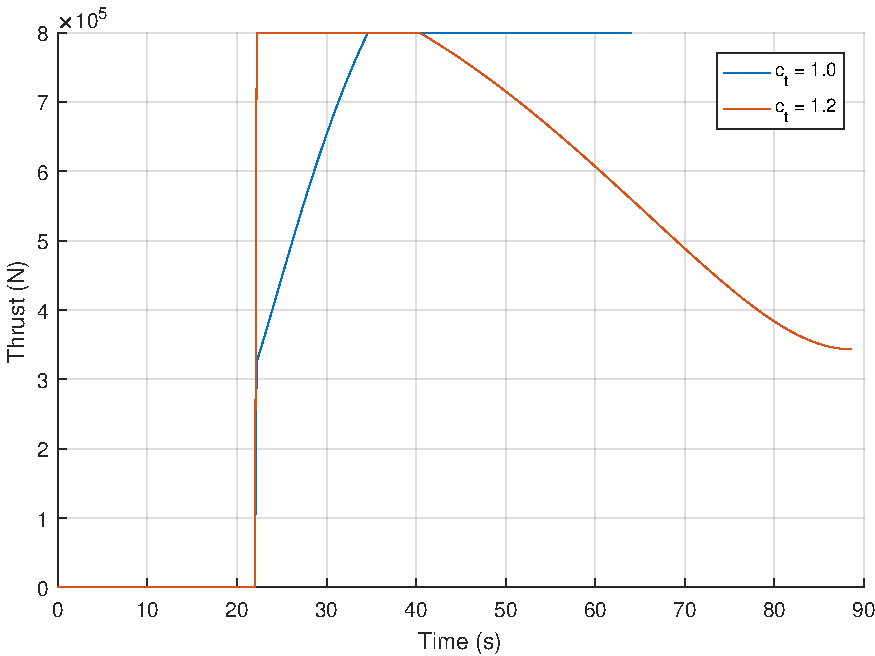
\includegraphics[width=\linewidth]{Figures/thrtgofac.pdf}
		\caption{PDI Time-to-go Factor: Thrust \label{fig:thrtgofac} }
	\end{minipage}
\end{figure}

\begin{figure}[H]
	\centering
	\begin{minipage}{4.5 in}
		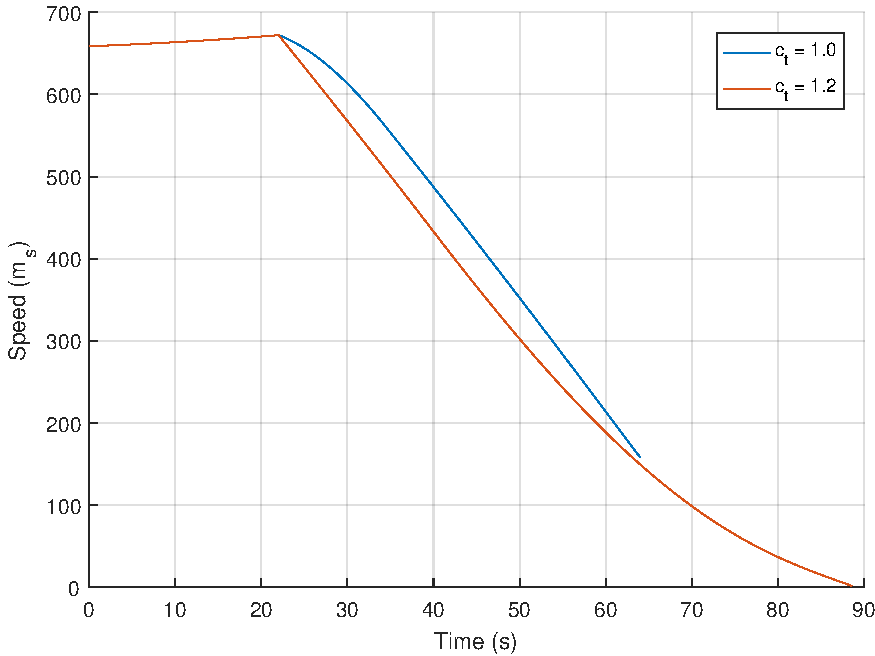
\includegraphics[width=\linewidth]{Figures/spdtgofac.pdf}
		\caption{PDI Time-to-go Factor: Speed \label{fig:spdtgofac} }
	\end{minipage}
\end{figure}



The second is the threshold values for the thrust acceleration and downrange criteria. Here these criteria are applied directly without modifying the threshold values; the powered descent initiation is triggered when the full maximum thrust or the full downrange distance is required for a gravity turn. But these thresholds can be raised or lowered. PDI can trigger when the thrust acceleration required exceeds some fraction of the maximum thrust acceleration available, or when the downrange distance to landing site is some multiple of the downrange distance required by a gravity turn. The exact relationship between these threshold values and the time-to-go factor $c_t$ is unknown and could be explored. 

